\documentclass[letterpaper, 10.5pt,landscape]{article}
\renewcommand{\familydefault}{\sfdefault} %% default font
\usepackage{multicol}
\usepackage{calc}
\usepackage{ifthen}

\usepackage[usenames,dvipsnames]{color}  % for text color


\usepackage[landscape]{geometry}
\usepackage[inkscapelatex=false]{svg}


\def\mathcolor#1#{\@mathcolor{#1}}
\def\@mathcolor#1#2#3{%
  \protect\leavevmode
  \begingroup
    \color#1{#2}#3%
  \endgroup
}

\usepackage[
backend=biber,
style=numeric,
sorting=ynt
]{biblatex}
\addbibresource{reference.bib}


\usepackage{ragged2e}
\usepackage{tabularx}


\usepackage{amsmath, amssymb, amsthm}
\usepackage{blkarray} % For block array
\DeclareMathOperator*{\argmin}{argmin}
\usepackage{latexsym, marvosym}
\usepackage{pifont}
\usepackage{lscape}
\usepackage{graphicx}
\usepackage{array}
\usepackage{booktabs}
\usepackage[bottom]{footmisc}
\usepackage{tikz}
\usetikzlibrary{shapes}
\usepackage{pdfpages}
\usepackage{wrapfig}
\usepackage{enumitem}
\setlist[description]{leftmargin=0pt}
\usepackage{xfrac}
\usepackage[pdftex,
            pdfauthor={William Chen},
            pdftitle={Probability Cheatsheet},
            pdfsubject={A cheatsheet pdf and reference guide originally made for Stat 110, Harvard's Introduction to Probability course. Formulas and equations for your statistics class.},
            pdfkeywords={probability} {statistics} {cheatsheet} {pdf} {cheat} {sheet} {formulas} {equations}
            ]{hyperref}
\usepackage[
            open,
            openlevel=2
            ]{bookmark}
\usepackage{relsize}
\usepackage{rotating}

 \newcommand\independent{\protect\mathpalette{\protect\independenT}{\perp}}
    \def\independenT#1#2{\mathrel{\setbox0\hbox{$#1#2$}%
    \copy0\kern-\wd0\mkern4mu\box0}} 
            
\newcommand{\noin}{\noindent}    
\newcommand{\logit}{\textrm{logit}} 
\newcommand{\var}{\textrm{Var}}
\newcommand{\cov}{\textrm{Cov}} 
\newcommand{\corr}{\textrm{Corr}} 
\newcommand{\N}{\mathcal{N}}
\newcommand{\Bern}{\textrm{Bern}}
\newcommand{\Bin}{\textrm{Bin}}
\newcommand{\Beta}{\textrm{Beta}}
\newcommand{\Gam}{\textrm{Gamma}}
\newcommand{\Expo}{\textrm{Expo}}
\newcommand{\Pois}{\textrm{Pois}}
\newcommand{\Unif}{\textrm{Unif}}
\newcommand{\Geom}{\textrm{Geom}}
\newcommand{\NBin}{\textrm{NBin}}
\newcommand{\Hypergeometric}{\textrm{HGeom}}
\newcommand{\HGeom}{\textrm{HGeom}}
\newcommand{\Mult}{\textrm{Mult}}




\geometry{top=.2in,left=.2in,right=.2in,bottom=.2in}

\pagestyle{empty}
\makeatletter
\renewcommand{\section}{\@startsection{section}{1}{0mm}%
                                {-1ex plus -.5ex minus -.2ex}%
                                {0.1ex plus .2ex}%x
                                {\normalfont\small}}
\renewcommand{\subsection}{\@startsection{subsection}{2}{0mm}%
                                {-1explus -.5ex minus -.2ex}%
                                {0.5ex plus .2ex}%
                                {\normalfont\normalsize\bfseries}}
\renewcommand{\subsubsection}{\@startsection{subsubsection}{3}{0mm}%
                                {-1ex plus -.5ex minus -.2ex}%
                                {1ex plus .2ex}%
                                {\normalfont\small\bfseries}}
\makeatother

\setcounter{secnumdepth}{0}

\setlength{\parindent}{0pt}
\setlength{\parskip}{0pt plus 0.5ex}

% -----------------------------------------------------------------------

\usepackage{titlesec}

\titleformat{\section}
{\color{teal}\normalfont\large\bfseries}
{\color{teal}\thesection}{1em}{}
\titleformat{\subsection}
{\color{teal}\normalfont\normalsize}
{\color{teal}\thesection}{1em}{}
\titleformat{\subsubsection}
{\color{teal}\normalfont\small}
{\color{teal}\thesection}{1em}{}

% Comment out the above 5 lines for black and white

\begin{document}

\raggedright
\footnotesize

\begin{multicols*}{3}

% multicol parameters
% These lengths are set only within the two main columns
%\setlength{\columnseprule}{0.25pt}
\setlength{\premulticols}{1pt}
\setlength{\postmulticols}{1pt}
\setlength{\multicolsep}{1pt}
\setlength{\columnsep}{2pt}

%%%%%%%%%%%%%%%%%%%%%%%%%%%%%%%%%%%%
%%% TITLE
%%%%%%%%%%%%%%%%%%%%%%%%%%%%%%%%%%%%

\begin{center}
    {\color{teal} \Large{\textbf{Probability \& Statistics}}} \\
   % {\Large{\textbf{Probability Cheatsheet}}} \\
    % comment out line with \color{blue} and uncomment above line for b&w
   \copyright \ 2024 \  Robins Yadav 
\end{center}



% Cheatsheet format from
% http://www.stdout.org/$\sim$winston/latex/

%%%%%%%%%%%%%%%%%%%%%%%%%%%%%%%%%%%%
%%% BEGIN CHEATSHEET
%%%%%%%%%%%%%%%%%%%%%%%%%%%%%%%%%%%%

% \href{https://github.com/robinyUArizona}{My github: https://github.com/robinyUArizona}








%%%%%%%%%%%%%%%%%%%%%%%%%%%%%%%%%%%%%%%%%%%%%%%%%%%%%%%%%%%%%
%%%%%% Probability %%%%%%%%%%%%%%%%%%%%%%%%%%%%%%%%%%

\section{Probability} {\color{teal}\hrule height 1pt} \smallskip

Probabilities A.K.A. Chance $\rightarrow$ How likely something (an event) is to happen? Probabilities \underline{ARE NOT} Guarantees! $\rightarrow$ Probability tells you that \textbf{over the long run} there is a certain chance of something happening, not that something will or will not happen at a specific time.

$\bullet$ Probability is a measure of the size of a set.


$\rightarrow$ Bridge between descriptive \& inferential statistics \\
$\rightarrow$ In \textbf{probability}, properties of the \textbf{population} are assumed known \& questions regarding a \textbf{sample} taken from the population are posed and answered. \\

\textcolor{blue}{Naive Definition of Probability} \\
If all outcomes are equally likely, the probability of an event $A$ happening is:
\[\boxed{P_{\textrm{naive}}(A) = \frac{\textnormal{number of outcomes favorable to $A$}}{\textnormal{number of outcomes}}}\]


\subsection{Counting} {\color{teal}\hrule height 0.5pt} \smallskip
\subsubsection{Multiplication Rule} {\color{teal}\hrule height 0.5pt} \smallskip
    \begin{minipage}{\linewidth}
            \centering
            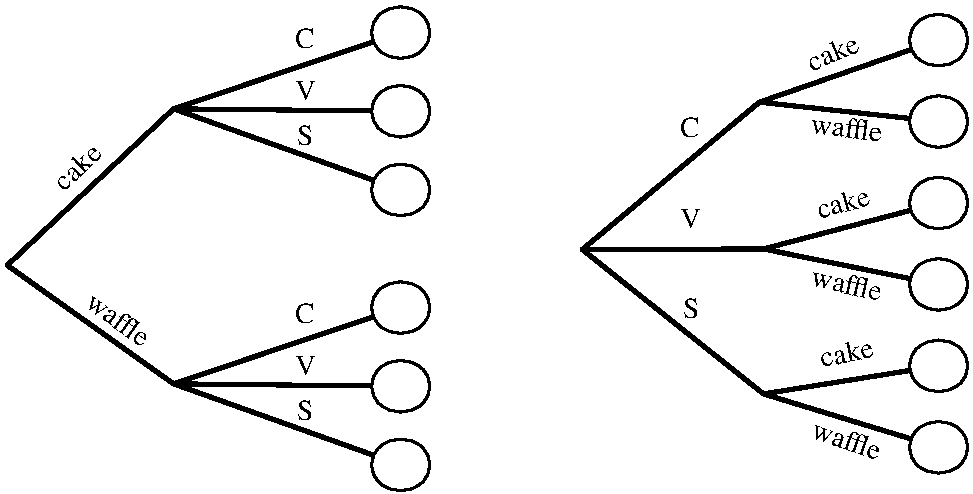
\includegraphics[width=2in]{figures/icecream.pdf}
        \end{minipage}
        
 Let's say we have a compound experiment (an experiment with multiple components). If the 1st component has $n_1$ possible outcomes, the 2nd component has $n_2$ possible outcomes, \dots, and the $r$th component has $n_r$ possible outcomes, then overall there are $n_1n_2 \dots n_r$ possibilities for the whole experiment.

\vspace{3pt}

\subsubsection{Permutation \& Combination} {\color{teal}\hrule height 0.5pt} \smallskip

% \href{https://www.youtube.com/watch?v=TYs6QQLTWIc&list=PLIYnk9FMYckuWpLCLVAVk50YyhZtaMFYr&index=39}{Video to add}



$\bullet$ \textbf{Permutation}: A permutation is an arrangement of $r$ objects from a pool of $n$ objects in a \textbf{given order}.


\vspace{-5pt}
\[\boxed{{}_n \mathrm{ P }_r = \frac{n!}{(n-r)!},  \hspace{20pt} 0\leq r \leq n}\]

\vspace{3pt}
$\rightarrow$ \textcolor{purple}{\textbf{Permutation when all the Objects are Distinct}} \\
\textbf{Theorem 1}: If the number of permutations of $n$ different objects taken $r$ at a time, satisfying the condition \(\boxed{0 < r \leq n} \), and where the \textbf{repetition is not allowed} is 
\vspace{-5pt}
\[\boxed{{}_n \mathrm{ P }_r \rightarrow \frac{n!}{(n-r)!} = n(n-1)(n-2) \cdots (n-r+1)} \]



\textbf{Theorem 2}: If the number of permutations of $n$ different objects taken $r$ at a time, where the \textbf{repetition is allowed }is
\vspace{-5pt}
\[\boxed{n^{r}} \]


\vspace{3pt}
$\rightarrow$  \textcolor{purple}{\textbf{Permutation when all the Objects are not Distinct}} \\
\textbf{Theorem 3}: The number of permutations of $n$ objects, and $p$'s are of the same kind and rest is all different kind is 
\vspace{-3pt}
\[\boxed{\frac{n!}{p!}}\]



\textbf{Theorem 4}: The number of permutations of $n$ objects, where $n_{1}$ are the objects of one kind, $n_{2}$ are of the second kind, ..., $n_{k}$ is of the $k^{\text{th}}$ kind and the rest, if any, are of a different kind, then the permutation is given by 
\vspace{-3pt}
\[\boxed{\frac{n!}{n_{1}! n_{2}! \cdots n_{k}!}} \]

\vspace{5pt}
$\bullet$ \textbf{Combination}:  A combination is an arrangement of $r$ objects from a pool of $n$ objects, where the \textbf{order does not matter}.\\
$\rightarrow$ We use combinations to count the number of ways to choose a group of $r$ unordered objects from $n$ possibilities \textbf{without replacement} by 
\vspace{-3pt}
\[\boxed{{}_n \mathrm{ C }_r = \frac{n!}{(n-r)! \hspace{3pt} r!} = \frac{{}_n \mathrm{ P }_r}{r!} = \frac{n(n-1)(n-2) \cdots (n-r+1)}{r!}} \]




$\rightarrow$ We use combinations to count the number of ways to choose a group of $r$ unordered objects from $n$ possibilities \textbf{with replacement} by
\vspace{-3pt}
\[\boxed{{}_n \mathrm{ C }_r = \frac{(r+n-1)!}{r! \hspace{3pt} (n-1)!}}\]



\textcolor{blue}{Note}: \textbf{without replacement} or \textbf{without repetition} means that you can \textbf{not} pick the same element more than once.


\vspace{-5pt}
%%%%%%%%%%%%%%%%%%%%%%%%%%%%%%%%%%%%%%%%%%%%%%%

% Examples of Tables
%\begin{table}[H]
\begin{center}
        \setlength{\extrarowheight}{5pt}
    \begin{tabular}{r|cc}
         & \textbf{Permutation} & \textbf{Combination}  \\ \hline
        \textbf{With Replacement} & $ n^k$ & $\frac{(r+n-1)!}{r! \hspace{3pt} (n-1)! \hspace{3pt}}$ \\
        \textbf{Without Replacement} & $\frac{n!}{(n - k)!}$ & $\frac{n!}{(n-r)! \hspace{3pt} r!}$
    \end{tabular}
\end{center}
%\end{table}
    

% \begin{center}
%     \begin{tabular}{ccc}
%         ~ & \textbf{Replace} & \textbf{No Replace}  \\
%     \midrule
%         \textbf{Fixed \# trials ($n$)} & Binomial & HGeom \\ 
%         ~ & (Bern if $n = 1$) & ~ \\ 
%         \textbf{Draw until $r$ success} & NBin & NHGeom \\ 
%         ~ & (Geom if $r = 1$) & ~\\ \bottomrule
%     \end{tabular}
% \end{center}




\subsection{Thinking Conditionally} {\color{teal}\hrule height 0.5pt} \smallskip
\subsubsection{Independence}{\color{teal}\hrule height 0.5pt} \smallskip

$\bullet$ \textbf{Independent Events}: Events $A$ and $B$ are \textbf{independent}, if and only if one of the following equivalent statements holds: 
\vspace{-5pt}
\begin{align*}
    & P(A \cap B) = P(A)P(B) \\
    & \hspace{8pt} P(A|B) = P(A) \\
    & \hspace{8pt} P(B|A) = P(B)
\end{align*}



$\bullet$ Events $A$, $B$, and $C$ are \textbf{mutually independent} if \textbf{both} of the following hold:\\
\hspace{5pt} (a) $A$, $B$, and $C$ are pairwise independent: 
\vspace{-5pt}
\begin{align*}
    P(A \cap B) = P(A)P(B) \\
    P(A \cap C) = P(A)P(C) \\
    P(B \cap C) = P(B)P(C)
\end{align*}

\vspace{-5pt}
\hspace{5pt} (b) \(P(A \cap B \cap C) = P(A)P(B)P(C) \)

\vspace{3pt}
$\bullet$ \textbf{Conditional Independence}:  Events ${A}$ and ${B}$ are \textbf{conditionally independent} given ${C}$ if $\boxed{P({A}\cap {B}|{C}) = P({A}|{C}) \hspace{3pt} P({B}|{C})}$. \\
$\rightarrow$ Conditional independence does not imply independence, and independence does not imply conditional independence.


\subsubsection{Unions, Intersections, and Complements}{\color{teal}\hrule height 0.5pt} \smallskip

\textbf{De Morgan's Laws}: A useful identity that can make calculating probabilities of unions easier by relating them to intersections, and vice versa. Analogous results hold with more than two sets.
\vspace{-3pt}
\begin{align*} 
\boxed{({A} \cup { B})^c = {A^c} \cap { B^c}} \\
\boxed{({A} \cap {B})^c = { A^c} \cup { B^c}}
\end{align*} 
                  
\textbf{Complements}: The following are true.
\vspace{-3pt}
\[\boxed{A \cup A^c = \Omega} \hspace{5pt} \boxed{A \cap A^c = \emptyset} \hspace{5pt} \boxed{P(A) = 1 -  P(A^c)} \]






\subsubsection{Joint Probability} {\color{teal}\hrule height 0.5pt} \smallskip

$\bullet$ The \textbf{joint probability} $P(A, B)$ or $P(A;B)$ is the probability of both $A$ and $B$ occurring simultaneously (same time).  
\vspace{-3pt}
 \[\boxed{P(A, B) = P(A \cap B)  = \frac{N(A \cap B)}{N(B)}} \]



\subsubsection{Conditional Probability}{\color{teal}\hrule height 0.5pt} \smallskip

\textbf{Conditional Probability}, with all outcomes equally likely. \\

$\bullet$ The \textbf{\textit{conditional} probability} of event $A$, given that event $B$ occurs is given by
\vspace{-3pt}
\[\boxed{P(A | B) = \frac{P(A \cap B)}{P(B)}}  \hspace{5pt} \rightarrow  \boxed{P(A \cap B) = P(B) \cdot P(A|B)}\]
\textbf{Note}: \(\boxed{P(A|B) \neq P(B|A)}\)


\vspace{5pt}

$\bullet$ \textbf{Law of Total Probability}: 
\vspace{-3pt}
\[\boxed{P(B) = \sum_{i=1}^{n} P(B|A_{i}) \hspace{2pt} P(A_{i})} \hspace{10pt} \boxed{\Omega = \bigcup \limits_{i=1}^{n} A_{i}}  \]


\subsubsection{Marginal Probability} {\color{teal}\hrule height 0.5pt} \smallskip

$\bullet$ The \textbf{marginal probability} is a $P(A)$; can compute by \textit{marginalizing} the \textit{joint distribution} $\mathcal{B} = \{B_{1}, B_{2}, ..., B_{n} \}$ is a collection of mutually exclusive events 
\vspace{-3pt}
 \[\boxed{P(A) = \sum \limits_{B \in \mathcal{B}} P(A,B) = \sum \limits_{B \in \mathcal{B}} P(A \cap B)}\]









\subsubsection{Bayes' Theorem}{\color{teal}\hrule height 0.5pt} \smallskip
The chance of you getting hit by lightning at the top of a tall building is high compared to on the ground. Hence information about the location changes the probability. Bayesian tries to interpret such additional information in terms of probability. Given your location, we can have a more precise probability of an event, than a "any location" or a "generic location".
\vspace{2pt}

For events $A$ and $B$ such that $P(B)>0$, we have
\vspace{-3pt}
\[\boxed{P(A|B) = \frac{P(B|A) \hspace{2pt} P(A)}  {P(B)}}  \]

\textbf{Note}: $P(A|B)$ and $P(B|A)$ are not the same thing!
\vspace{-5pt}

\[\boxed{P(A_{i}|B) = \frac{P(B|A_{i}) \hspace{2pt}
P(A_{i})}{\sum_{j=1}^{n}P(B|A_{j}) \hspace{2pt} P(A_{j})}}  \hspace{10pt} \boxed{\Omega = \bigcup \limits_{i=1}^{n} A_{i}} \]



\textbf{Likelihood and Posterior} 
\vspace{-5pt}
\[\mathcolor{orange}{P(A|B)} = \frac{\mathcolor{green}{P(B|A)} \, \mathcolor{purple}{P(A)}} {P(B)} \]
\vspace{-10pt}

• \mathcolor{purple}{$P(A)$} is the \textcolor{purple}{prior}
\\
• \mathcolor{green}{$P(B | A)$} is the \textcolor{green}{likelihood}  \\
• $P(B) = \int P(B|A) P(A) \hspace{2pt} dA $ is a scaling factor (constant $A$) \\
• $\mathcolor{orange}{P(A|B)}$ is the \textcolor{orange}{posterior}.




Bayesian probability is like a logic of probability, where we walk from the initial hypothesis (prior) to final beliefs through premises (likelihood) and observations (data).


















\subsection{Probability space} {\color{teal}\hrule height 0.5pt} \smallskip

A probability space, \textbf{a mathematical concept}, is a ordered triple \((\Omega,\mathcal{B}, \mathrel{P})\), respectively the \textit{sample space}, \textit{event space}, and \textit{probability function}. \\



$\Omega$: \textbf{sample space} $\rightarrow$ Set of outcomes of an experiment.\\
\textcolor{blue}{Example}: tossing a coin twice. $\Omega = \{\text{HH, HT, TH, TT}\}$ \\

\vspace{5pt}
$\mathcal{B}$: \textbf{event space} $\rightarrow$ all possible \textbf{subsets} of an \textbf{sample space} $\Omega$. An event is a subset of $\Omega$ \\
\textcolor{blue}{Example}: (i) "at least one head" is $\{\text{HH, HT, TH} \}$, (ii) "no more than one head" is $\{\text{HT, TH, TT} \}$ \\
\vspace{3pt}
In \textbf{probability theory}, the event space $\mathcal{B}$ is modelled as a \textbf{$\sigma$-algebra} (or\textbf{ $\sigma$-field}) of $\Omega$, which is a collection of subsets of $\Omega$ with the following properties: \\
(1) \( \boxed{\emptyset \in \mathcal{B}} \) \\
(2) If an event \( \boxed{A \in \mathcal{B}} \), then \(\boxed{A^{\complement} \in \mathcal{B}} \) (closed under complementation) \\
(3) If \( \boxed{A_{1}, A_{2},... \in \mathcal{B}} \), then \( \boxed{\bigcup \limits_{i=1}^{\infty} A_{i} \in \mathcal{B} }\) (closed under countable union). \\

\vspace{2pt}
\textbf{Additional properties}:\\
(4) (1) + (2) $\rightarrow$ \( \boxed{\Omega \in \mathcal{B}} \) \\
(5) (3) + De-Morgan's Laws $\rightarrow$ \( \boxed{\bigcap \limits_{i=1}^{\infty} A_{i} \in \mathcal{B} }\) (closed under countable intersection)


\textcolor{blue}{Example}: tossing a coin twice \\
\(\Omega = \{\text{HH, HT, TH, TT}\}\), then \(  \mathcal{B} = 2^{\Omega} = 16\), and therefore \textbf{ $\sigma$-field} can be given by \( \{\emptyset, \{HH\}, \{HT\}, \{TH\}, \{TT\}, \{HH, HT\}, \{HH, HT, TH\}, \cdots , \Omega  \}\)

\textcolor{red}{\textbf{Note}:} Observable events could be the collection of all intervals, plus what can be obtained by set operations \(\cup, \cap, \complement \).

\vspace{3pt}
Suppose we cannot distinguish between \(\text{HT} \) and \(\text{TH}\), then we have sample space \(\Omega = \{\text{HH, HT, TT} \}\), and \(\mathcal{B} = 2^{\Omega} = 8\), therefore \textbf{ $\sigma$-field} can be given by \( \{\emptyset, \{HH\}, \{HT\}, \{TT\}, \{HH, HT\}, \{HH, TT\}, \{HT, TT\}, \Omega  \}\)

\vspace{3pt}
\textcolor{blue}{Example}: (i) "at least one head" is $\{\text{HH, HT, TH} \}$. \\
If we want the smallest $\sigma$-\textbf{field} that makes $\{\text{HH, HT, TH} \}$ measurable, then qualitatively $\sigma$-\textbf{field} formed by taking complements, finite intersections, and countable unions of members of \(\mathcal{B}\), until it satisfies all requirements of a $\sigma$-\textbf{field}. When we go through this process, we obtain the $\sigma$-\textbf{algebra},
\(\mathcal{B} = \{\emptyset, \{TT\},  \{HH, HT, TH\}, \cdots , \Omega  \ \})\)






\vspace{5pt}
$\mathrel{P}$: \textbf{probability measure} $\rightarrow$ a function that assigns numbers (called probabilities) between $0$ and $1$ to each event in $\mathcal{B}$ i.e. \( \mathcal{B} \rightarrow [0,1] \) \\
In other words, a \textbf{probability measure} is a function
\( \boxed{P : \mathcal{B} \rightarrow [0,1]}\)  that maps an event $A$ to a real number in \( [0,1]\). The function must satisfy the \textbf{axioms of probability}: \\

\vspace{2pt}

\textbf{\textcolor{blue}{Probability Axioms}} \\
1. \textbf{Non-negativity}: \(\boxed{P(A) \geq 0 }\), for all \(A \in \mathcal{B} \) $\rightarrow$ ensures that probability is never negative. \\
2. \textbf{Normalization}: \(\boxed{P(\Omega) = 1}\).   $\rightarrow$ ensures that probability is never greater than 1.\\
3. Countable \textbf{Additivity}: If \( A_{1}, A_{2}, ... \in \mathcal{B} \) are pairwise disjoint (i.e., \(A_{i} \cap A_{j} = \emptyset \), if $i\neq j$), then
\(\boxed{P \left( \bigcup \limits_{i=1}^{\infty} A_{i} \right) = \sum \limits_{i=1}^{\infty} P(A_{i})}\)


\textcolor{blue}{\textbf{Theorem}:} Let \((\Omega,\mathcal{B}, \mathrel{P})\) be a probability space. \\
1. \(\mathrel{P}(A^{\complement}) = 1 - \mathrel{P}(A) \hspace{5pt} \text{for} \hspace{5pt} A \in \mathcal{B}\)\\
2. \(\mathrel{P}(A \cup B)  =  \hspace{3pt} \mathrel{P}(A) + \mathrel{P}(B) - \mathrel{P}(A \cap B). \hspace{5pt} \text{for} \hspace{5pt} A, B \in \mathcal{B}\)\\
3. \( \mathrel{P}(A/B) = \hspace{3pt} \mathrel{P}(A) - \mathrel{P}(A \cap B). \hspace{5pt} \text{for} \hspace{5pt} A, B \in \mathcal{B}\)\\
4. \(\text{If} \hspace{5pt} A \subset B, \hspace{5pt} \text{then} \hspace{5pt} \mathrel{P}(A) \leq \mathrel{P}(B) \hspace{5pt} \text{for} \hspace{5pt} A,B \in \mathcal{B}\)\\
5.  If \( A_{1}, A_{2}, ... \in \mathcal{B} \) are disjoint, then  
\(\boxed{P \left( \bigcup \limits_{j=1}^{n} A_{j} \right) = \sum \limits_{j=1}^{n} P(A_{j})}\)


\vspace{3pt}
\textcolor{blue}{Example}:: Tossing a coin twice. Assuming that the coin is fair, then the \textit{probability function} for the $\sigma$-algebra consisting of all subsets of $\Omega$ is 

\begin{minipage}{0.8\linewidth}
% \begin{figure}[h!]
    \centering
    % \begin{minipage}[b]{0.75\textwidth}
    \includegraphics[width=\textwidth]{figures/Probability_Space_Example.PNG}
    % \caption{ML Production}
    % \label{fig:ML_Production}
    % \end{minipage}
% \end{figure}
\end{minipage}

\textcolor{blue}{Example}:: A coin toss.\\
\(\Omega: \{\text{H, T}\} \) \\
\(\mathcal{B}: \big\{\phi, \{\text{H}\}, \{\text{T}\}, \{\text{H, T}\}  \big\} \) \\
$\mathrel{P}$: \( P(\phi) = 0, \hspace{5pt} P(\{ \text{H}\}) = \frac{1}{4}, \hspace{5pt} P(\{ \text{T}\}) = \frac{3}{4}, \hspace{5pt} P(\{\text{H,T}\}) = 1 \)
\\

























\subsection{Random Variable} {\color{teal}\hrule height 0.5pt} \smallskip

Consider an experiment with four outcomes \(\Omega = \{ \clubsuit, \diamondsuit, \heartsuit, \spadesuit \}\). We want to construct the probability space \( \left( \Omega, \mathcal{B}, P \right)\). The sample space $\Omega$ is already defined. The event space $\mathcal{B}$ is the set of all possible subsets in $\Omega$, which, in our case, is a set of $2^{4}$ subsets. For the probability law $P$, let us assume that the probability of obtaining each outcome is \vspace{-5pt}
\[P[\{\clubsuit\}] = \frac{1}{6}, \hspace{3pt} P[\{\diamondsuit\}] = \frac{2}{6}, \hspace{3pt} P[\{\heartsuit\}] = \frac{2}{6}, \hspace{3pt} P[\{\spadesuit\}] = \frac{1}{6}\].

\vspace{-5pt}

Therefore, we have constructed a \textbf{probability space} \( \left( \Omega, \mathcal{B}, P \right)\) where everything is perfectly defined. So, in principle, they can live together happily forever. \\
A lazy data scientist comes, and there is a (small) problem. The data scientist does not want to write the symbols $\clubsuit$, $\diamondsuit$, $\heartsuit$, $\spadesuit$. There is nothing wrong with his motivation because all of us want efficiency. How can we help him? Well, the easiest solution is to encode each symbol with a number, for example, $\clubsuit \leftarrow 1$,  $\diamondsuit \leftarrow 2$,
$\heartsuit \leftarrow 3$,
$\spadesuit \leftarrow 4$, where the arrow that we assign a number to the symbol. But we can express this more formally by defining a function \( \boxed{X: \Omega \rightarrow \mathbb{R}}\) with 
\vspace{-5pt}

\[X(\clubsuit) = 1, \hspace{3pt} X(\diamondsuit) = 2, \hspace{3pt}  X(\heartsuit) = 3, \hspace{3pt}
X(\spadesuit) = 4\]  



There is nothing new here: we have merely converted the symbols to numbers, with the help of a function X, However, with X defined, the probabilities can be written as
\vspace{-3pt}
\[P[X=1] = \frac{1}{6}, \hspace{3pt} P[X=2] = \frac{2}{6}, \hspace{3pt} P[X=3] = \frac{2}{6}, \hspace{3pt} P[X=4] = \frac{1}{6}\]
\vspace{-3pt}
This is much more convenient, and so the data scientist is happy.


\vspace{7pt}

A \textbf{random variable} $X$ on a probability space \( \left( \Omega, \mathcal{B}, P \right)\) is a function that maps every element in a sample space to a real line i.e.,\(\boxed{X: \Omega \rightarrow \mathbb{R}} \)

\vspace{2pt}

In other words, A random variable is a rule that assigns a numerical value to each outcome in a sample space. \\


\vspace{5pt}
\textcolor{blue}{Example}: Flip a coin 2 times. The sample space $\Omega$ is 
\vspace{-3pt}
\[\Omega = \{(\text{head, head}), (\text{head, tail}), (\text{tail, head}), (\text{tail, tail})\}\]

Suppose that $X$ is a random variable that maps an outcome to a number representing the sum of "head", i.e,
\[X(\cdot) = \text{number of heads}.\]

Then, for the four $\xi$'s in the sample space there are only 3 distinct numbers. More precisely, if we let $\xi_{1} = (\text{head, head}), \xi_{2} = (\text{head, tail}), \xi_{3} = (\text{tail, head}), \xi_{4} = (\text{tail, tail})$, then, we have
\vspace{-2pt}
\[X(\xi_{1}) = 2, \hspace{3pt} X(\xi_{2}) = 1, \hspace{3pt} X(\xi_{3}) = 1, \hspace{3pt} X(\xi_{4}) = 0\]

This shows that the mapping defined by the random variable is not necessarily a one-to-one mapping because multiple outcomes can be mapped to the same number.

\begin{center}
    \begin{minipage}{\linewidth}
    \includegraphics[width=0.9\textwidth]{figures/randomVariable_mapping.PNG}
    \end{minipage}
\end{center}







\vspace{5pt}

\subsubsection{Types of Random Variables} {\color{teal}\hrule height 0.5pt} \smallskip
(1) \textbf{Numerical RV} \\
\hspace{5pt} (i) Discrete RV: can take only distinct, separate values \\
\hspace{5pt} (ii) Continuous RV: can take any value in some interval (low, high) \\
(2) \textbf{Categorical RV} \\


\subsection{Probability Distribution Functions} {\color{teal}\hrule height 0.5pt} \smallskip

\textbf{\textcolor{blue}{Probability Distribution}}: describes how the probability of $\Omega$ is distributed along the range of $X$. \\
$\rightarrow$ The probability distribution of $X$ says how the total probability of 1 is distributed among the various possible $X$ values. \\



\begin{center}
\begin{tabular}{cc}
\hline
\textbf{Command} & \textbf{What it does} \\
\hline
\texttt{help(distributions)} & shows documentation on distributions\\
\texttt{dbinom(k,n,p)} & PMF $P(X=k)$ for $X \sim \Bin(n,p)$\\
\texttt{dt(x,n)} & PDF $f(x)$ for $X \sim t_n$\\
\texttt{dunif(x,a,b)} & PDF $f(x)$ for $X \sim \Unif(a,b)$\\
\hline
\end{tabular}
\end{center}


\vspace{3pt}
Let $X$ have pmf $f(x)$ then, here $f(x)$  is \(\boxed{p_{X}(x) = P[X=x]}\).
\scalebox{0.80}{
                        \setlength{\extrarowheight}{7pt}
            \begin{tabular}{ccc}
                  \textbf{Discrete $X$} & \textbf{Continuous $X$} \\
            \toprule
            $\boxed{\mu = E(X) = \sum \limits_{i=1}^{n} xf(x)} $ & $\boxed{\mu = E(X) =\int \limits_{-\infty}^\infty xf(x) \hspace{2pt} dx}$ \\
            $\boxed{\sigma_{X}^{2} = V(X) = \sum \limits_{i=1}^{n} \left(x-\mu \right)^{2} f(x)}$ & 
            $\boxed{\sigma_{X}^{2} = V(X) = \int \limits_{-\infty}^{\infty} \left(x-\mu \right)^{2} f(x) \hspace{2pt} dx}$\\
            $\boxed{\sigma_{X}^{2} = E\left[(X-\mu)^2\right] = E(X^{2}) - \left[E(X) \right]^{2}}$  & fvd \\
            \bottomrule
            \end{tabular}
        }
        \medskip


        
$\bullet$ Properties of Variance
\begin{enumerate}
	\item $\boxed{V(aX + b) = a^2 \cdot \sigma^2}$
	\item In particular, $\boxed{\sigma_{aX} = |a| \cdot \sigma_{x}}$
	\item $\boxed{\sigma_{X+b} = \sigma_{X}}$
\end{enumerate}        





\vspace{5pt}


\subsubsection{Probability Mass Functions (PMF)} {\color{teal}\hrule height 0.5pt} \smallskip
The \textbf{PMF} gives the probability of a discrete random variable $X$ that takes on the value $x$ i.e, $X(\xi) = x$. $\rightarrow$ The set of all possible states of $X$ is denoted as $X(\Omega)$ \\ We denote PMF as 
\vspace{-3pt}
\[ \boxed{p_{X}(x) = P[X=x]}\]

\vspace{-7pt}
\begin{center}
    \begin{minipage}{0.7\linewidth}
        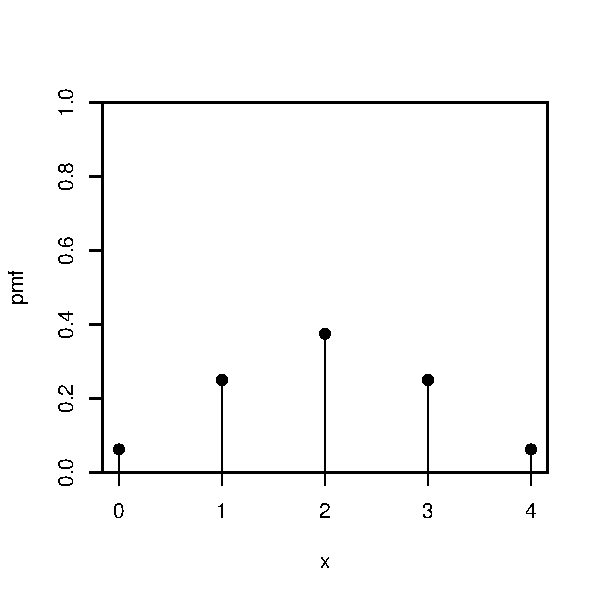
\includegraphics[width=\textwidth]{figures/Binpmf.png}
        % \caption{ML Production}
        % \label{fig:ML_Production}
    \end{minipage}
\end{center}

\vspace{-7pt}
The PMF satisfies,\\
\(p_{X}(x) \geq 0, \hspace{5pt} \text{and}  \hspace{5pt} \sum_{x} p_{X}(x) = 1\)


\vspace{3pt}
% $\rightarrow$ Probabilities for any interval, also called \textbf{probability mass}: \\
% $\rightarrow$ $\boxed{P(x_{1} \leq X < x_{2}) = F(x_{2}) - F(x_{1})}$ \\


$\rightarrow$ The \textbf{probabilities} are summarized by a function known as the probability mass function (PMF). \\
$\rightarrow$ PMFs are the ideal histograms of random variables. \\

$\rightarrow$ \(\boxed{\text{Expectation} = \text{Mean} = \text{Average computed from a PMF}} \)

\vspace{5pt}
\textcolor{blue}{Example}: Flip a coin twice. The sample space is $\Omega = \{\text{HH, HT, TH, TT}\}$. We can assign a random variable $X =\text{number of heads}$. Therefore,
\vspace{-3pt}
\[X(\text{"HH"}) = 2, \hspace{3pt} X(\text{"TH"})=1, \hspace{3pt}
X(\text{"HT"})=1, \hspace{3pt}
X(\text{"TT"})=0 \].

\vspace{-7pt}

So the random variable $X$ takes three states: 0,1,2. The PMF is therefore
\vspace{-5pt}
\[p_{X}(0) = P[X=0] = P[\{\text{"TT"} \}] = \frac{1}{4}, \]
\vspace{-5pt}
\[p_{X}(1) = P[X=1] = P[\{\text{"TH", "HT"} \}] = \frac{1}{2}, \]
\vspace{-5pt}
\[p_{X}(2) = P[X=2] = P[\{\text{"HH"} \}] = \frac{1}{4} \]

$\rightarrow$ The PMF is the weighing function for discrete random variables. Two random variables are different when their PMFs are different because they are constructing two different measures.


\vspace{3pt}
\subsubsection{Cumulative Density Function (CDF)}{\color{teal}\hrule height 0.5pt} \smallskip
The CDF gives the probability that a random variable $X$ is less than or equal to $x$.
\[F_X(x) = P(X \leq x)\]
\vspace{-5pt}
\begin{center}
    \begin{minipage}{0.7\linewidth}
        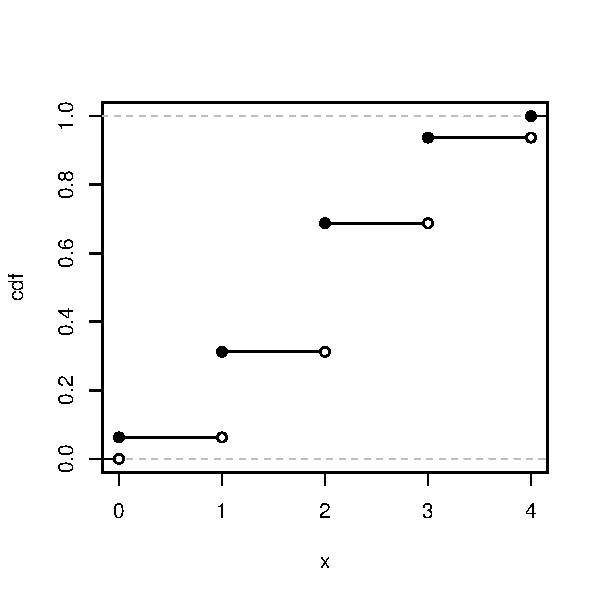
\includegraphics[width=\textwidth]{figures/Bincdf.png}
        % \caption{ML Production}
        % \label{fig:ML_Production}
    \end{minipage}
\end{center}
\vspace{-5pt}



The CDF is an increasing, right-continuous function with
\[F_X(x) \to 0 \textrm{ as $x \to -\infty$ and } F_X(x) \to 1 \textrm{ as $x \to \infty$} \]




$\bullet$ Continuous probabilities $F_{X}$, \textbf{CDF}:
$\rightarrow$ \( F_{X}(x) = P[X \leq x] \),  monotonic, non-decreasing, x goes to $\infty$
\begin{center}
    \begin{minipage}{\linewidth}
    \includegraphics[width=0.9\textwidth]{figures/CDF_probability.PNG}
    \end{minipage}
\end{center}

\textbf{What's the probability that a Continuous Random Variables is in an interval?} Take the difference in CDF values (or use the PDF as described later).
\[\boxed{P(a \leq X \leq b) = P(X \leq b) - P(X \leq a) = F_X(b) - F_X(a)}\]

For $X \sim \N(\mu,\sigma^2)$, this becomes
\begin{align*}
P(a\leq X\leq b)&=\Phi \left(\frac{b-\mu }{\sigma } \right) - \Phi \left( \frac{a-\mu }{\sigma } \right)
\end{align*}


\vspace{5pt}
\textbf{\textcolor{blue}{Example}:} Consider a random variable $X$ with PMF $p_{X}(0) = \frac{1}{4}, p_{X}(1) = \frac{1}{2} \hspace{3pt} \text{and} \hspace{3pt} p_{X}(4) = \frac{1}{4} $. The CDF of $X$ can be computed as 
\vspace{-5pt}

\begin{align*}
    F_{X}(0) & = P[X \leq 0] = p_{X}(0) = \frac{1}{4}, \\
     F_{X}(1) &  = P[X \leq 1] = p_{X}(0) + p_{X}(1)  = \frac{3}{4}, \\
      F_{X}(4) &  = P[X \leq 4] = p_{X}(0) + p_{X}(1) + p_{X}(4)  = 1
\end{align*}

\vspace{-5pt}

\begin{center}
    \begin{minipage}{\linewidth}
    \includegraphics[width=0.9\textwidth]{figures/PMF_CDF_RandomVariables.PNG}
    \end{minipage}
\end{center}

$\bullet$ Converting between PMF and CDF: If $X$ is a discrete random variable, then the PMF of $X$ can be obtained from the CDF by \[\boxed{p_{X}(x_{k}) = F_{X}(x_{k}) - F_{X}(x_{k-1})}\]
\vspace{-5pt}

Continue the above example 
\vspace{-5pt}
    \[p_{X}(0) = F_{X}(0) - F_{X}(-\infty) = \frac{1}{4} - 0 = \frac{1}{4}, \]
    \[p_{X}(1) = F_{X}(1) - F_{X}(0) = \frac{1}{4} - 0 = \frac{3}{4} - \frac{1}{4} = \frac{1}{2}, \]
    \[p_{X}(4) = F_{X}(4) - F_{X}(1) = 1-\frac{3}{4} = \frac{1}{4}.\]



\subsubsection{Probability Density Function (PDF)}{\color{teal}\hrule height 0.5pt} \smallskip

The PDF $f$ is the derivative of the CDF $F$.
\[ F'(x) = f(x) \]
A PDF is nonnegative and integrates to $1$. By the fundamental theorem of calculus, to get from PDF back to CDF we can integrate:
\begin{align*} 
    F(x) &=  \int_{-\infty}^x f(t)dt  
   \end{align*}
   
   
\begin{center}
    \begin{minipage}{\linewidth}
    \includegraphics[width=0.9\textwidth]{figures/Logisticpdfcdf.PNG}
    \end{minipage}
\end{center}   


   
Let $X$ be a continuous random variable. The  PDF of $X$ is a function \(f_{X}: \Omega \rightarrow \mathbb{R}\) that, when integrated over an interval $[a,b]$ yields the probability of obtaining $a \leq X \leq b:$
\[\boxed{\mathbb{P}[a\leq X \leq b] = F(b) - F(a) = \int_{a}^{b} f_{X}(x) \hspace{2pt} dx} \]



Two additional properties of a PDF:  it must integrate to 1 (because the probability that a CRV falls in the interval $[-\infty, \infty]$ is 1, and the PDF must always be non-negative.
\[\int^\infty_{-\infty}f(x)dx = 1 \hspace{2 cm} f(x) \geq 0\]



\textcolor{blue}{Example}: Let $f_{X}(x) = 3x^{2}$ with $\Omega = [0,1]$. Let $A=[0,0.5]$. The probability $\mathbb{P}[\{X \in A \}]$ is 
\vspace{-3pt}
\[\mathbb{P}[0 \leq X \leq 0.5] = \int_{0}^{0.5} 3x^{2} \hspace{2pt} dx = \frac{1}{8}\]




$\rightarrow$ Densities can exceed 1, $\rightarrow$ Densities are \textbf{not} probabilities. \\

\textbf{Note}: \textit{Continous distributions \textbf{does not} have probability mass functions} instead we use \textbf{probability density} because the probability of a continuous variable being any one precise value is 0.

\textbf{\textcolor{blue}{Note:} } The PDF and the CDF of a given random variable contain exactly the same information.









\subsubsection{Classic Statistical Distribution}{\color{teal}\hrule height 0.5pt} \smallskip

$\bullet$ \textcolor{purple}{Binomial Distribution} (\textbf{Discrete}): $x$ successes in $n$ independent trials or events, each with $p$ probability. Here, each success occurs with the same probability $p$ and each failure occurs with probability $1-p$. \textbf{Example}: Used in quality control and polling. Assume $X$ is distributed \(\text{Bin}(n,p) \). 
\vspace{-3pt}
\[\boxed{\text{PDF: } P(X=x) =  \binom{n}{x}  p^x (1-p)^{n-x} \quad : x = 0,1,2,\ldots }\]
\vspace{-5pt}
\[\boxed{\mu = np} \hspace{10pt} \boxed{\sigma^{2} = np(1-p)}\]


\vspace{-4pt}
\begin{center}
    \begin{minipage}{0.5\linewidth}
    \includegraphics[width=\textwidth]{figures/binomial_prob_distribution.jpg}
    \end{minipage}
\end{center}
\vspace{-4pt}


\textcolor{purple}{Negative Binomial}:  
Number of failures before $r$ successes. \\

\vspace{3pt}
$\bullet$ \textcolor{purple}{Bernoulli Distribution}:  if $n=1$, this is a Bernoulli distribution. \\
\textbf{Example}: Binary outcomes like flipping a coin, yes/no surveys
\[\boxed{\mu = p} \hspace{10pt} \boxed{\sigma^{2} = p(1-p)}\]

\vspace{-4pt}
\begin{center}
    \begin{minipage}{0.5\linewidth}
    \includegraphics[width=\textwidth]{figures/bernouli_prob_distribution.jpg}
    \end{minipage}
\end{center}
\vspace{-4pt}

\vspace{3pt}


\vspace{3pt}
$\bullet$ \textcolor{purple}{Geometric}: 
$1^{st}$ success with $p$ probability on the $n$ trails. Tracks visits before the first Ad click
\vspace{-3pt}
\[\boxed{\text{PDF: } P(X=x) = q^{n-1}p} \hspace{15pt} \boxed{\mu = \frac{1}{p}} \hspace{15pt} \boxed{\sigma^{2} = \frac{1-p}{p^2}} \]

\textcolor{purple}{Hypergeometric}: 
$x$ successes in $n$ draws, no replacement, from a size $N$ population with $X$ items of that feature
\vspace{-3pt}
\[\boxed{\text{PDF: } P(X=x) = \frac{ \binom{X}{x} \binom{N-X}{n-x}} {{\binom{N}{n}}}} \hspace{15pt} \boxed{\mu = \frac{nX}{N}} \]







$\bullet$ \textcolor{purple}{Poisson Distribution} (\textbf{Discrete}):  Counts in fixed intervals. \textbf{Example}: No. of calls received per call center. Assume $X$ is distributed \(\text{Pois}(\lambda) \). Number of $x$ successes in a fixed interval of time/space, where these success occur independently and with a known constant or average rate $\lambda$.

\vspace{-3pt}
\[\boxed{\text{PDF: } P(x) = \frac{e^{-\lambda} \lambda^{x}}{x!}} \hspace{15pt}  \boxed{\mu =   \lambda} \hspace{15pt} \boxed{\sigma^{2} = \lambda }  \]

\vspace{-4pt}
\begin{center}
    \begin{minipage}{0.5\linewidth}
    \includegraphics[width=\textwidth]{figures/poisson_prob_distribution.jpg}
    \end{minipage}
\end{center}
\vspace{-4pt}

$\bullet$ \textcolor{purple}{Power Law Distribution} (\textbf{Discrete}):
Many data distributions have much longer tails than
the normal or Poisson distributions. In other words,
the change in one quantity varies as a power of another
quantity. It helps measure the inequality in the world.
e.g. wealth, word frequency and Pareto Principle (80/20
Rule)
\vspace{-3pt}
\[\boxed{\text{PDF: } P(X=x) = cx^{-\alpha}}\]
where $\alpha$ is the law's exponent and $c$ is the normalizing constant.


\vspace{3pt}
$\bullet$ \textcolor{purple}{Uniform Distribution} (\textbf{Continuous}):
All values have equal probabilities. \textbf{Example}:  Used in random number generator

\[\boxed{\text{PDF: } P(x) = \frac{1}{b-a}} \hspace{15pt} \boxed{\mu =\frac{a+b}{2}}  \hspace{15pt}  \boxed{\sigma^{2} = \frac{(b-a)^{2}}{12} } \]


\vspace{-4pt}
\begin{center}
    \begin{minipage}{0.5\linewidth}
    \includegraphics[width=\textwidth]{figures/uniform_prob_distribution.jpg}
    \end{minipage}
\end{center}
\vspace{-4pt}


\vspace{3pt}
$\bullet$ \textcolor{purple}{Normal/Gaussian Distribution} (\textbf{Continuous}): \\
Assume $X$ in distributed $\mathcal{N}(\mu, \sigma^{2})$. It is a bell-shaped and symmetric distribution. Bulk of the values lie close to the mean and no value is too extreme. Generalization of the binomial distribution as $n \rightarrow \infty$.
\vspace{-3pt}
\[\boxed{\text{PDF: } P(x) = \frac{1}{\sigma\sqrt{2\pi}} e^-\frac{(x-\mu)^{2}}{2\sigma^{2}}} \hspace{15pt} \boxed{\mu =\mu}  \hspace{15pt}  \boxed{\sigma^{2} =  \sigma^{2}} \]


\textbf{Implications}: 68\%-95\%-99\% rule. 68\% of probability mass fall within 1$\sigma$ of the mean, 95\% within 2$\sigma$, and 99.7\% within 3$\sigma$.


$\rightarrow$ Normal Approximation - discrete distributions such as Binomial and Poisson can be approximated using $z$-scores when $np$, $nq$, and $\lambda$ are greater than 10.
\vspace{-4pt}
\begin{center}
    \begin{minipage}{0.5\linewidth}
    \includegraphics[width=\textwidth]{figures/normal_prob_distribution.jpg}
    \end{minipage}
\end{center}
\vspace{-4pt}



\vspace{2pt}
$\bullet$ \textcolor{purple}{Exponential} -  Time between events. \textbf{Example}: Explains inactivity time among users. 
Memoryless time  between independent event occuring at an average rate $\boxed{\lambda \rightarrow \lambda e^{\lambda x}}$, with $\boxed{\mu = \frac{1}{\lambda}}$
\vspace{-4pt}
\begin{center}
    \begin{minipage}{0.5\linewidth}
    \includegraphics[width=\textwidth]{figures/exponential_prob_distribution.jpg}
    \end{minipage}
\end{center}
\vspace{-4pt}




\vspace{2pt}

$\bullet$ \textcolor{purple}{Gamma} -  Time between K-th success. \textbf{Example}: Explains load on web servers over time. Time until $n$ independent events occuring at an average rate $\lambda$.



\subsection{Joint PDFs and CDFs} {\color{teal}\hrule height 0.5pt} \smallskip

\subsubsection{Joint Distributions}{\color{teal}\hrule height 0.5pt} \smallskip
The \textbf{joint CDF} of $X$ and $Y$ is 
$$\boxed{F(x,y)=P(X \leq x, Y \leq y)}$$
In the discrete case, $X$ and $Y$ have a \textbf{joint PMF} 
$$\boxed{p_{X,Y}(x,y) = P(X=x,Y=y)}$$ In the continuous case, they have a \textbf{joint PDF}
\[\boxed{f_{X,Y}(x,y) = \frac{\partial^2}{\partial x \partial y} F_{X,Y}(x,y)}\]
The joint PMF/PDF must be nonnegative and sum/integrate to 1.
\begin{minipage}{\linewidth}
            \centering
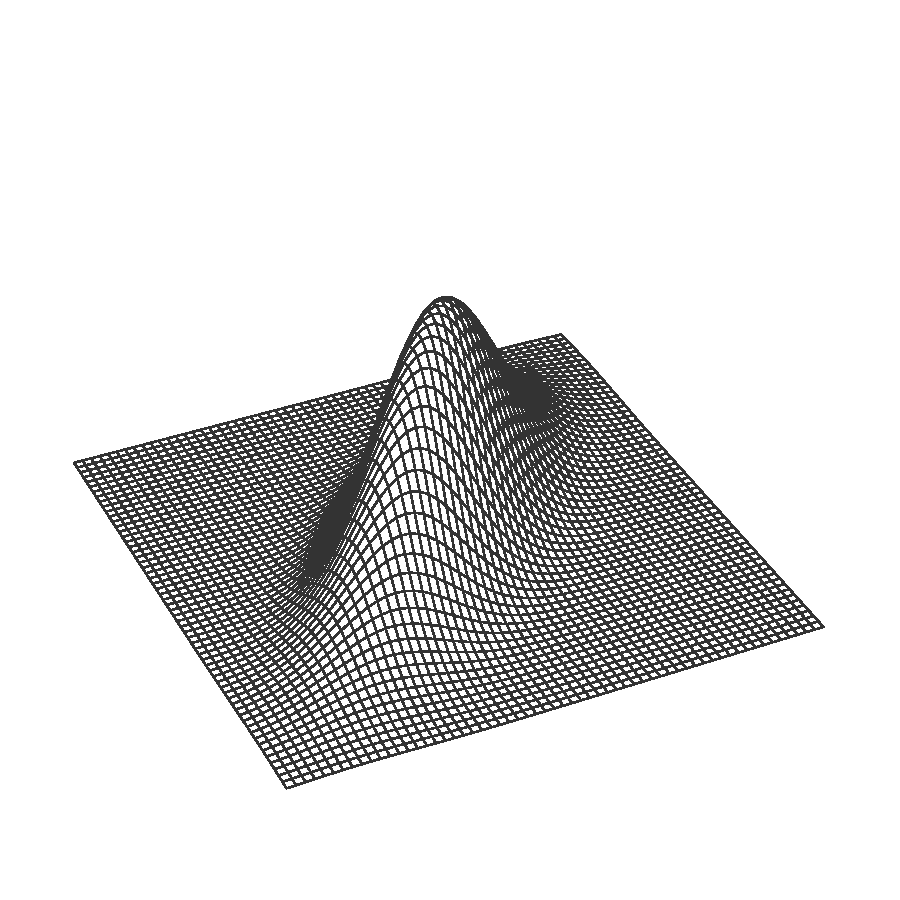
\includegraphics[width=1.0in]{figures/jointPDF.pdf}
        \end{minipage}

\subsubsection{Conditional Distributions} {\color{teal}\hrule height 0.5pt} \smallskip    
\textbf{Conditioning and Bayes' rule for discrete r.v.s}
\vspace{-5pt}
\[\boxed{P(Y=y|X=x) = \frac{P(X=x, Y=y)}{P(X=x)} = \frac{P(X=x|Y=y)P(Y=y)}{P(X=x)}}\]
\textbf{Conditioning and Bayes' rule for continuous r.v.s}
\vspace{-5pt}
\[\boxed{f_{Y|X}(y|x) = \frac{f_{X,Y}(x, y)}{f_X(x)} = \frac{f_{X|Y}(x|y)f_Y(y)}{f_X(x)}}\]
\textbf{Hybrid Bayes' rule}
\vspace{-5pt}
\[\boxed{f_X(x|A) = \frac{P(A | X = x)f_X(x)}{P(A)}}\]


\subsubsection{Marginal Distributions}{\color{teal}\hrule height 0.5pt} \smallskip
To find the distribution of one (or more) random variables from a joint PMF/PDF, sum/integrate over the unwanted random variables.

\textbf{Marginal PMF from joint PMF}
\vspace{-5pt}
\[\boxed{P(X = x) = \sum_y P(X=x, Y=y)}\]
\textbf{Marginal PDF from joint PDF}
\vspace{-5pt}
\[\boxed{f_X(x) = \int_{-\infty}^\infty f_{X, Y}(x, y) dy}\]

\textbf{\textcolor{blue}{Independence of Random Variables}}  
Random variables $X$ and $Y$ are independent if and only if any of the following conditions holds:
\vspace{-3pt}
\begin{itemize}
    \itemsep -1mm
    \item Joint CDF is the product of the marginal CDFs 
    \item Joint PMF/PDF is the product of the marginal PMFs/PDFs
    \item Conditional distribution of $Y$ given $X$ is the marginal distribution of $Y$
\end{itemize}
 Write $X \independent Y$ to denote that $X$ and $Y$ are independent.
 

\subsubsection{Expectation}{\color{teal}\hrule height 0.5pt} \smallskip
The expected value of a function $h(X, Y)$ of two jointly distributed random variables is  
\vspace{-5pt}
$$ \boxed{	E(g(X,Y)) = \sum_{x\in \mathbb{D}_1} \sum_{y\in \mathbb{D}_2} g(x,y)p(x,y)}	$$
\vspace{-5pt}
and can be generalized to the continuous case with integrations.

\vspace{5pt}


\subsection{Correlation} {\color{teal}\hrule height 0.5pt} \smallskip

$\bullet$ \textbf{Variance: } is a numerical value that describes the \textbf{variability} of observations from its arithmetic mean. \\
% The \textbf{variabiltiy} is the extent to which data points in a statistical distribution or data set diverge—vary—from the average value, as well as the extent to which these data points differ from each other.\\
\textcolor{blue}{Note:} The more spread the data, the larger the variance is in relation to the mean.
\vspace{-5pt}
\[\boxed{\sigma^{2} = \frac{\sum(x_{i} - \mu)^{2}}{n} = E\left[ \left(X - E[X] \right)^{2} \right]} \]


$\bullet$ \textbf{Standard deviation: } is a measure of the \textbf{dispersion} of observations within a data set.
\vspace{-3pt}
\[\boxed{\sigma = \sqrt{\text{variance}}} \]

\textbf{Key points: }

\begin{enumerate}
    \vspace{-3pt}
    \item Both variance and standard deviation are always positive.
    \vspace{-3pt}
    \item If all the observations in a data set are identical, then the standard deviation and variance will be zero.
    \vspace{-3pt} 
    \item Standard deviation is preferred over mean as it is expressed in the same units as those of the measurements while the variance is expressed in the units larger than the given data set
\end{enumerate}


$\bullet$ \textbf{Covariance: } measures the \textbf{direction} of a relationship between two variables.\\
Covariance is a quantitative measure of the extent to which the deviation of one variable from its mean matches the deviation of the other from its mean.  \\

Ex.: When two stocks tend to move together, they are seen as having a positive covariance; when they move inversely, the covariance is negative.
\vspace{-5pt}
\[\boxed{\text{Cov}(X,Y) = E \left[\left(X - E[X] \right)  \left( Y- E[Y]  \right)   \right]} \]
\vspace{-3pt}
Special case: \(\boxed{\sigma^{2} = \text{Cov}(X, X)  }\) 

\vspace{5pt}

$\bullet$ \textbf{Correlation:} measures the \textbf{strength} of the linear relationship between two variables. It is normalized version of covariance.
\vspace{-3pt}
\[\boxed{\text{Cor}(X, Y) = \frac{\text{Cov}(X,Y)}{\sigma_{X} \sigma_{Y}}} \]

Pearson Correlation: $-1 \leq r \leq 1$, Range [-1, 1] $\rightarrow$ 0 is uncorrelated


For a sample: 
\vspace{-5pt}
\[\boxed{r = \frac{\sum(x_{i} - \bar{x}) (y_{i} - \bar{y})}{\sqrt{\sum (x_{i} - \bar{x})^{2}} \sqrt{\sum(y_{i} - \bar{y})^{2}}}} \]



\begin{minipage}{\linewidth}
% \begin{figure}[h!]
    \centering
    % \begin{minipage}[b]{0.75\textwidth}
    \includegraphics[width=\textwidth]{figures/Correlation_example_figures.PNG}
    % \caption{ML Production}
    % \label{fig:ML_Production}
    % \end{minipage}
% \end{figure}
\end{minipage}

\textbf{Correlation and Independence} \\
$\rightarrow$ Two random variables are \textbf{independent} are uncorrelated i.e. \(\boxed{\text{Corr}(X, Y) = 0} \), if $P(X|Y) = P(X)$. Also, This is because if $X$
 and $Y$ are independent, then one property is \(E[XY] = E[X]E[Y]\)


$\rightarrow$ Reverse is not necessarily true - some uncorrelated variables are dependent





\subsection{Law of Large Numbers (LLN)} {\color{teal}\hrule height 0.5pt} \smallskip

The LLN states that if you sample a random variable independently a large number of times, the measured average value should converge to the random variable's true expectation.
\vspace{-3pt}
\[\boxed{\bar{X}_{n} = \frac{X_{1} + \ldots + X_{n}}{n} \rightarrow \mu, \hspace{5pt} \text{as} \hspace{3pt} n \rightarrow \infty}\]
This is important in studying the longer-term behavior of random variables over time. As an example, a coin might land on heads 5 times in a row, but over a much larger $n$ we would expect the proportion of heads to be approximately half of the total flips. Similarly, a casino might experience a loss on any individual game, but over the long run should see a predictable profit over time.



\subsection{Central Limit Theorem (CLT)} {\color{teal}\hrule height 0.5pt} \smallskip

The CLT states that if you repeatedly sample a random variable a large number of times, the distribution of the sample mean will approach a normal distribution regardless of the initial distribution of the random variable. The normal distribution takes on 
\vspace{-3pt}
\[\boxed{f_{X}(x) = \frac{1}{\sqrt{2\pi\sigma^{2} }} \text{exp}-\left(\frac{(x-\mu)^{2}}{2\sigma^{2}} \right)}\] 
\vspace{-3pt}
with the mean $\mu$ and standard deviation $\sigma$ respectively. \\


\vspace{5pt}
The CLT states that: 
\vspace{-3pt}
\[\boxed{\bar{X}_{n} = \frac{X_{1} + \ldots + X_{n}} {n} \rightarrow \hspace{5pt} \sim N\left(\mu, \frac{\sigma^{2}}{n} \right) ; \hspace{5pt}}\]  
\vspace{-5pt}
hence,
\vspace{-5pt}
\[\boxed{\frac{\bar{X}_{n} - \mu}{\frac{\sigma}{\sqrt{n}}} \sim N(0,1)}\]

At a very basic level, you can consider the implications of this theorem on coin flipping: the probability of getting some number of heads flipped over a large $n$ should be approximately that of a normal distribution. \\

\textbf{\textcolor{blue}{Note:}} Whenever you are asked to reason about any particular distribution over a large sample size, you should remember to think of the CLT, regardless of whether it is Binomial, Poisson, or any other distribution.



\subsection{Markov Chains} {\color{teal}\hrule height 0.5pt} \smallskip
 Markov chain is a mathematical system that experiences transitions from one state to another according to certain probabilistic rules. The defining characteristic of a Markov chain is that no matter how the process arrived at its present state, the possible future states are fixed. In other words, the probability of transitioning to any particular state is dependent solely on the current state and time elapsed. The state space, or set of all possible states, can be anything: letters, numbers, weather conditions, baseball scores, or stock performances.


Ref: \href{https://www.youtube.com/playlist?list=PLX2gX-ftPVXWgcF0WATMDr-AfvfaYjJZ3}{Markov Chain Tutorial}

\vspace{-3pt}
\[\boxed{\left[\text{Next State}\right] = 
\begin{bmatrix}
\text{Matrix of}\\
\text{Transition}  \\
\text{Probabilities}
\end{bmatrix}
\left[\text{Current State} \right]
}\]

\[X_{1} = PX_{0}\]

\vspace{-3pt}
\begin{center}
    \begin{minipage}{0.6\linewidth}
    \includegraphics[width=\textwidth]{figures/Markov_chain_intro.PNG}
    \end{minipage}
\end{center}


\vspace{-5pt}
\[ \begin{bmatrix}
A_{1} \\
B_{1} \\
C_{1}
\end{bmatrix} = 
\begin{blockarray}{cccc}
A & B & C \\
\begin{block}{[ccc]c}
  0.8 & 0.2 & 0.1 & \hspace{-7pt}A \\
  0.1 & 0.7 & 0.3 & \hspace{-7pt}B \\
  0.1 & 0.1 & 0.6 & \hspace{-7pt}C \\
\end{block}
\end{blockarray}
\begin{bmatrix}
A = 200 \rightarrow 0.4 \\
B = 120 \rightarrow 0.24\\
C = 180 \rightarrow 0.36
\end{bmatrix}
=  \begin{bmatrix}
202 \rightarrow 0.404 \\
158 \rightarrow 0.316 \\
140 \rightarrow 0.28
\end{bmatrix}
\]

% \vspace{-5pt}
% \[ [A_{1} \quad B_{1} \quad C_{1}] = [A \quad B \quad C]
% \begin{blockarray}{cccc}
% \quad & A & B & C \\
% \begin{block}{c[ccc]}
%   A \hspace{5pt} & 0.8 & 0.1 & 0.1 \\
%   B \hspace{5pt} & 0.2 & 0.7 & 0.1  \\
%   C \hspace{5pt} & 0.1 & 0.3 & 0.6   \\
% \end{block}
% \end{blockarray}
% \]


\textcolor{purple}{\textbf{Why they call it chains
?}}
\vspace{-3pt}
\[X_{1} = PX_{0} \quad X_{2} = PX_{1} \quad X_{3} = PX_{2} \]

\vspace{-5pt}
\[ X_{2} = 
\begin{bmatrix}
  0.8 & 0.2 & 0.1 \\
  0.1 & 0.7 & 0.3 \\
  0.1 & 0.1 & 0.6 \\
\end{bmatrix}
\begin{bmatrix}
0.404 \\
0.316 \\
0.28
\end{bmatrix}
=
\begin{bmatrix}
0.414 \\
0.346 \\
0.240
\end{bmatrix} 
= 
\begin{bmatrix}
207 \\
173 \\
120
\end{bmatrix}
\]


\vspace{-3pt}
\[ X_{3} = 
\begin{bmatrix}
  0.8 & 0.2 & 0.1 \\
  0.1 & 0.7 & 0.3 \\
  0.1 & 0.1 & 0.6 \\
\end{bmatrix}
\begin{bmatrix}
0.414 \\
0.346 \\
0.240
\end{bmatrix} 
=
\begin{bmatrix}
0.424 \\
0.356 \\
0.220
\end{bmatrix} 
= 
\begin{bmatrix}
212 \\
178 \\
110
\end{bmatrix}
\]


\textbf{Another method to calculate chain:}
\vspace{-3pt}
\[X_{n} = P^{n}X_{0} \quad \rightarrow \quad X_{2} = P^{2}X_{0}, \quad X_{3} = P^{3}X_{0} \]

When chain continues, it may end of up with same stable distribution matrix i.e., $X_{s} = X_{s-1}$
\vspace{-3pt}
\[ X_{s} = PX_{s-1} = 
\begin{bmatrix}
  0.8 & 0.2 & 0.1 \\
  0.1 & 0.7 & 0.3 \\
  0.1 & 0.1 & 0.6 \\
\end{bmatrix}
\begin{bmatrix}
  \text{val}1 \\
  \text{val}4 \\
  \text{val}5
\end{bmatrix} =
\begin{bmatrix}
  \text{val}1 \\
  \text{val}4 \\
  \text{val}5
\end{bmatrix}
\] 




\subsubsection{Definition} {\color{teal}\hrule height 0.5pt} \smallskip

\begin{center}
    \begin{minipage}{\linewidth}
    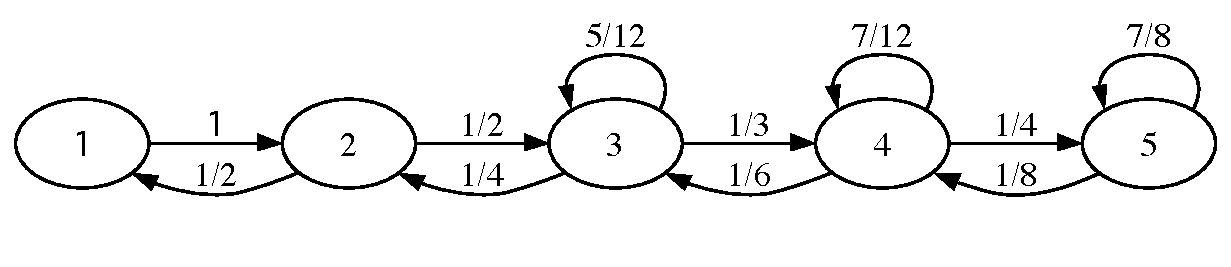
\includegraphics[width=\textwidth]{figures/chainA.pdf}
    \end{minipage}
\end{center}

A Markov chain is a random walk in a \textbf{state space}, which we will assume is finite, say $\{1, 2, \dots, M\}$. We let $X_t$ denote which element of the state space the walk is visiting at time $t$. The Markov chain is the sequence of random variables tracking where the walk is at all points in time, $X_0, X_1, X_2, \dots$. By definition, a Markov chain must satisfy the \textbf{Markov property}, which says that if you want to predict where the chain will be at a future time, if we know the present state then the entire past history is irrelevant.  \emph{Given the present, the past and future are conditionally independent}. In symbols,
\[P(X_{n+1} = j | X_0 = i_0, X_1 = i_1, \dots, X_n = i) = P(X_{n+1} = j | X_n = i)\]


\subsubsection{State Properties}{\color{teal}\hrule height 0.5pt} \smallskip
A state is either recurrent or transient.
\begin{itemize}
\item If you start at a \textbf{recurrent state}, then you will always return back to that state at some point in the future.  \textmusicalnote \emph{You can check-out any time you like, but you can never leave.}  \textmusicalnote
\item Otherwise you are at a \textbf{transient state}. There is some positive probability that once you leave you will never return. \textmusicalnote \emph{You don't have to go home, but you can't stay here.} \textmusicalnote
\end{itemize}
A state is either periodic or aperiodic.
\begin{itemize}
\item If you start at a \textbf{periodic state} of period $k$, then the GCD of  the possible numbers of steps it would take to return back is  $k>1$.
\item Otherwise you are at an \textbf{aperiodic state}. The GCD of  the possible numbers of steps it would take to return back is 1.
\end{itemize}


\subsubsection{Transition Matrix}{\color{teal}\hrule height 0.5pt} \smallskip
Let the state space be $\{1,2,\dots,M\}$. The transition matrix $Q$ is the $M \times M$ matrix where element $q_{ij}$ is the probability that the chain goes from state $i$ to state $j$ in one step:
\[q_{ij} = P(X_{n+1} = j | X_n = i)\]

To find the probability that the chain goes from state $i$ to state $j$ in exactly $m$ steps, take the $(i, j)$ element of $Q^m$.
\[q^{(m)}_{ij} = P(X_{n+m} = j | X_n = i)\]
If $X_0$ is distributed according to the row vector PMF $\vec{p}$, i.e., $p_j = P(X_0 = j)$, then the PMF of $X_n$ is $\vec{p}Q^n$.



\subsubsection{Chain Properties} {\color{teal}\hrule height 0.5pt} \smallskip
A chain is \textbf{irreducible} if you can get from anywhere to anywhere. If a chain (on a finite state space) is irreducible, then all of its states are recurrent. A chain is \textbf{periodic} if any of its states are periodic, and is \textbf{aperiodic} if none of its states are periodic. In an irreducible chain, all states have the same period. \medskip

A chain is \textbf{reversible} with respect to $\vec{s}$ if $s_iq_{ij} = s_jq_{ji}$ for all $i, j$.  Examples of reversible chains include any chain with $q_{ij} = q_{ji}$, with $\vec{s} = (\frac{1}{M}, \frac{1}{M}, \dots, \frac{1}{M})$, and random walk on an undirected network.


\subsubsection{Stationary Distribution}{\color{teal}\hrule height 0.5pt} \smallskip

Let us say that the vector $\vec{s} = (s_1, s_2, \dots, s_M)$ be a PMF  (written as a row vector). We will call $\vec{s}$ the \textbf{stationary distribution} for the chain if $\vec{s}Q = \vec{s}$. As a consequence, if $X_t$ has the stationary distribution, then all future $X_{t+1}, X_{t + 2}, \dots$ also have the stationary distribution. \\

\smallskip

For irreducible, aperiodic chains, the stationary distribution exists, is unique, and $s_i$ is the long-run probability of a chain being at state $i$. The expected number of steps to return to $i$ starting from $i$ is $1/s_i$.

\smallskip

 To find the stationary distribution, you can solve the matrix equation $(Q' - I){\vec{s}\,}'= 0$. The stationary distribution is uniform if the columns of $Q$ sum to 1.



\textbf{Reversibility Condition Implies Stationarity}  If you have a PMF $\vec{s}$ and a Markov chain with transition matrix $Q$, then $s_iq_{ij} = s_jq_{ji}$ for all states $i, j$ implies that $\vec{s}$ is stationary.





\subsubsection{Random Walk on an Undirected Network}{\color{teal}\hrule height 0.5pt} \smallskip


\begin{center}
    \begin{minipage}{0.5\linewidth}
    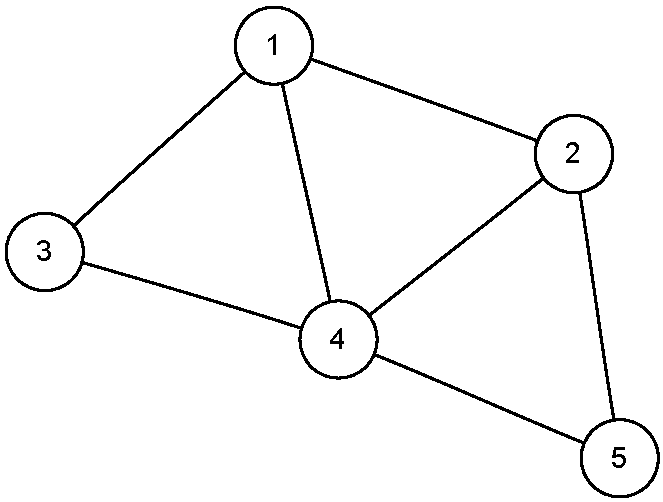
\includegraphics[width=\textwidth]{figures/network1.pdf}
    \end{minipage}
\end{center}




If you have a collection of \textbf{nodes}, pairs of which can be connected by undirected \textbf{edges}, and a Markov chain is run by going from the current node to a uniformly random node that is connected to it by an edge, then  this is a random walk on an undirected network. The stationary distribution of this chain is proportional to the \textbf{degree sequence} (this is the sequence of degrees, where the degree of a node is how many edges are attached to it). For example, the stationary distribution of random walk on the network shown above is proportional to $(3,3,2,4,2)$, so it's $(\frac{3}{14}, \frac{3}{14}, \frac{2}{14}, \frac{4}{14}, \frac{2}{14})$. 

\vspace*{\fill}




\pagebreak


%%%%%%%%%%%%%%%%%%%%%%%%%%%%%%%%%%%%%%%%%%%%%%%%%%%%%%%%%%%%%
%%%%%% Statistcs %%%%%%%%%%%%%%%%%%%%%%%%%%%%%%%%%%


\section{Statistics} {\color{teal}\hrule height 1pt} \smallskip

\subsection{Descriptive Statistics:} {\color{teal}\hrule height 0.5pt} \smallskip

Used to describe, organize and summarize information about an entire population i.e. 90\% satisfaction of all customers.

$\bullet$ \textbf{\textcolor{purple}{Where is the variable centered?}} called \textit{\textbf{measure of central of tendency}}.\\

$\rightarrow$ \textbf{Mean}: Outliers draw the \textbf{mean} towards them! (also effect SD), critical for computation and prediction. For a dataset $x_1, x_2, \dots, x_n$
\vspace{-3pt}
\[\boxed{\mu = \frac{1}{n} \sum_{i=1}^{n} x_i}\]
 \vspace{-3pt}


$\rightarrow$ \textbf{Median}: increases with increase in small values, \textbf{good for heavily skewed data} or large outliers
\vspace{-3pt}
\[
\boxed{\text{Median} = 
\begin{cases} 
x_{\frac{n+1}{2}} & \text{if } n \text{ is odd} \\
\frac{x_{\frac{n}{2}} + X_{\frac{n}{2} + 1}}{2} & \text{if } n \text{ is even}
\end{cases}}
\]
\vspace{-3pt}

$\rightarrow$ \(\text{\textbf{Mode}} = \text{value that appears most frequently}\)

\vspace{5pt}
$\bullet$ \textbf{\textcolor{purple}{How spread out the data is?}} called \textit{\textbf{measure of variability}} 


$\rightarrow$ \textbf{Variance}: measures how far the values in a dataset spread out from the mean (average).
\vspace{-3pt}
\[
\boxed{
\sigma^2 = \frac{1}{n} \sum_{i=1}^{n} (x_i - \mu)^2
}
\]

$\rightarrow$ \textbf{Standard Deviation}: Variance gives extra weight to outliers due to Squared values, an interpretable measure of spread because it is expressed in the same units as the data.
\vspace{-3pt}
\[
\boxed{
\sigma = \sqrt{\sigma^2}
}
\]

$\rightarrow$ \textbf{Coefficient of Variation (CV)}: measures the relative variability of a dataset by comparing the standard deviation to the mean.
\vspace{-3pt}
\[\boxed{\text{CV} = \frac{\sigma}{\mu} \times 100\%}\]


$\rightarrow$ \textbf{Covariance}: measure of the degree to which two random variables change together. It indicates the \textbf{direction} of the linear relationship between the variables.
\vspace{-3pt}
\[\boxed{\text{Cov}(X, Y) = \frac{1}{n} \sum_{i=1}^{n} (x_i - \mu_X)(y_i - \mu_Y)}\]
\hspace{10pt}-  A positive covariance indicates that as one variable increases, the other also tends to increase. \\
\hspace{10pt}- A negative covariance indicates that the other tends to decrease as one variable increases. \\
\hspace{10pt}- A covariance close to zero suggests that the variables do not have a linear relationship.

$\rightarrow$ \textbf{Correlation Coefficients}: measures the \textbf{strength} and \textbf{direction} of a linear relationship between two variables. The formula for Pearson's correlation coefficient is:
\vspace{-3pt}
\[
\boxed{r = \frac{\sum (x_i - \bar{x})(y_i - \bar{y})}{\sqrt{\sum (x_i - \bar{x})^2 \sum (y_i - \bar{y})^2}}}
\]

The value of $r$ ranges from $-1$ to $1$: \\
\hspace{10pt}- $r = 1$: Perfect positive correlation.  \\
\hspace{10pt}- $r = -1$: Perfect negative correlation. \\
\hspace{10pt}- $r = 0$: No correlation.


$\rightarrow$ \textbf{Inter-quartile range: } width of "middle 50\%".
\(\text{IQR} = Q3 - Q1\)

\(\text{lower bound} = Q1 - 1.5 * \text{IQR}, \hspace{5pt}
\text{upper bound} = Q3 + 1.5 * \text{IQR}\)



\subsubsection{Types of Datasets} {\color{teal}\hrule height 0.5pt} \smallskip

\begin{itemize}
    \item \textbf{Structured} Ex: Table format i.e. based on row(s) and column(s)
    \vspace{-3pt}
    \item \textbf{Unstructured} Ex: unknown form - music, video, audio 
    \vspace{-3pt}
    \item \textbf{Semi-structured} Ex: JSON, CSV, XML, graph data, @email
    \vspace{-3pt}
\end{itemize}


\subsubsection{Types of Variables} {\color{teal}\hrule height 0.5pt} \smallskip

The level of measurement of your data determines which statistical tests are appropriate to use. 


$\rightarrow$  \textbf{Quantitative} $\rightarrow$ Numerical 
\begin{itemize}[leftmargin=0.8cm]
    \vspace{-3pt}
    \item \textbf{Continuous:} can take on any value (in allowable range). \\ \textbf{Ex}: A player's height (176.5cm), distance from KTM to JNK (200km)    
    \begin{itemize}[leftmargin=0.4cm]
        \vspace{-3pt}
        \item \textbf{Interval} - Measurable, but arbitrary zero point \\
        (\textbf{Note}: zero point is a point where all values start) \\
        \textbf{Ex}: credit scores (300-850)
        \vspace{-3pt}
        \item \textbf{Ratio} - Measurable and meaningful zero point. \\
        \textbf{Ex}: Weight, length, Temp. in Kelvin (in this scale zero marks the point, cannot go below it)
        \vspace{-3pt}
    \end{itemize}
    \item \textbf{Discrete:} takes on distinct (whole numeric) values. \\ $\rightarrow$ \textbf{Integers} are discrete. \textbf{Ex:} score in a soccer game (5 goals), how many siblings? (3 siblings), 
\end{itemize}

$\rightarrow$ \textbf{Qualitative} $\rightarrow$ Categorical (Descriptive) 
\begin{itemize}[leftmargin=0.8cm]
 \vspace{-3pt}
    \item \textbf{Nominal}: Categories with no ranking or natural order. All options have the \textbf{same} value. \\
    \textbf{Ex}: Gender, Ethnicity, Personal preferences (favorite meal or color),
     \vspace{-3pt}
    \item \textbf{Ordinal}: Categories with an inherent rank or order. Each options has a \textbf{different} value. \\
    \textbf{Ex}: Income levels (low, medium, high), Levels of agreement (Agree, Neutral, Disagree)
     \vspace{-3pt}
\end{itemize}



\vspace{5pt}

\subsubsection{Presentation} {\color{teal}\hrule height 0.5pt} \smallskip
$\bullet$ The goal of data presentation to communicate what we learned from the data, the evidence for our conclusions\\

\vspace{2pt}


$\rightarrow$ 3 primary ways to compare statistics: \textbf{absolute}, \textbf{relative}, and \textbf{ratio} \\
\vspace{2pt}

$\bullet$ \textbf{Bar chart: } Emphasize \textit{relative difference}. A bar chart is used for \textbf{categorical} data, where each bar represents a distinct category with variable heights indicating values like counts or percentages. It has a \textbf{categorical x-axis} and a \textbf{numerical y-axis}, showing comparisons between different categories (e.g., sales figures for different products).
% \vspace{1.8pt}


$\bullet$ \textbf{Histogram: } It displays the distribution of \textbf{numerical} data across bins or intervals. Bars are contiguous and represent the frequency or count of data points within each bin on the x-axis. It has numerical axes (x for bins, \textbf{y for frequencies}), helping visualize data distributions (e.g., exam scores distribution).
\vspace{2pt}


$\bullet$ \textbf{Box plot: }The distribution of a numeric variable within groups identified by a categorical variable. \\
\vspace{2pt}

$\bullet$ \textbf{Scatter plot: } Where observations fall in a two-dimensional space defined by two numeric variables \\
\vspace{2pt}

$\bullet$ \textbf{line plot: } How a numeric variable changes from one value to the next of another numeric variable \\
\vspace{2pt}


$\bullet$ \textbf{Point plot: } Emphasize \textit{absolute difference}, also relative difference-in-difference \\
\vspace{2pt}




$\bullet$ \textbf{Violin plot: } like box, but mean-based \\
\vspace{2pt}
$\bullet$ \textbf{Swarm plot: } categorical scatter plot \\
\vspace{2pt}




\subsection{Inferential Statistics} {\color{teal}\hrule height 0.5pt} \smallskip

Used to generalize about a population \textbf{based on a sample of data} i.e. 90\% satisfaction from a sample of 50 customer $\rightarrow$ 90\% satisfaction from all customers. 
\vspace{2pt}

\textbf{Inference} is learning about data \\
$\rightarrow$  \textbf{Estimating} the value of a parameter \\
$\rightarrow$ \textbf{Testing} the data's support for an hypothesis. \\


$\rightarrow$ \textbf{Ex:}  Mean of 500 penguins is \textbf{estimate } (is an estimated value often has a \textbf{CI} or similar), mean as the concept is the \textbf{estimator}, and the parameter is \textbf{estimand} \\

\vspace{2pt}
$\bullet$ \textbf{Sampling Distribution}: refers to the distribution of a \textbf{sample} statistic (such as the sample mean or sample proportion) obtained from \textbf{multiple samples of the same size} from a population. \\

\vspace{2pt}
$\bullet$ \textbf{Bootstrap}: A technique for \textbf{estimating sampling distributions} by repeatedly resampling the available (existing) sample \textbf{with replacement}.


\vspace{2pt}
$\bullet$ \textbf{Central Limit Theorem} (CLT) states that the sampling distribution of the sample mean approaches a \textbf{normal distribution} as sample size increases, regardless of the population \textbf{distribution} (i.e. uniform, exponential etc), given that the sample consists of independent and identically distributed i.e. i.i.d random variables with \textbf{finite} mean and variance.
\vspace{-4pt}
\[\boxed{Z_n = \frac{\bar{X}_n - \mu}{\frac{\sigma}{\sqrt{n}}} \xrightarrow{d} N(0, 1)
}\]
\vspace{-4pt}

The standardized sample mean $Z_{n}$ converges to a standard normal distribution $N(0,1)$ as the sample size 
$n$ increases.

$\rightarrow$ When we perform experiments or collect data, we often don't know the underlying distribution of the population (it could be \textbf{skewed}, \textbf{uniform}, or anything else). This is where the \textbf{Central Limit Theorem} (CLT) becomes crucial.


$\bullet$ \textbf{Sample statistic}: 
A metric calculated for a sample of data drawn from a large population.

$\bullet$ \textbf{Standard error} Measures the accuracy of the estimate \( \text{SE} = \frac{s}{\sqrt{n}}\)

\vspace{3pt}
$\rightarrow$ \textcolor{purple}{\textbf{QQ-Plot}}: A plot to visualize how close a sample distribution is to a specified distribution, e.g., the normal distribution


% \vspace{2pt}

\subsubsection{Normal Distribution} {\color{teal}\hrule height 0.5pt} \smallskip

We can compute the Z Score and use the Normal Distribution to calculate probabilities


\vspace{2pt}
$\bullet$ \textbf{Z-score}: gives the value in standard deviation ($\sigma$) for the Percentile we want. For example, if we want 95\% of the data, it tell us how many standard deviations are required. 
\vspace{-4pt}
\[\boxed{
Z = \frac{x - \mu}{\sigma}
}\]
\vspace{-4pt}

$\bullet$ \textbf{Z Table}: Area in Blue is $0.9803$ of the area
\vspace{-4pt}
\begin{center}
    \begin{minipage}{0.46\linewidth}
    \includegraphics[width=\textwidth]{figures/z_normal_distribution.jpg}
    \end{minipage}
\end{center}
\vspace{-4pt}
\vspace{-4pt}
\[\boxed{
Z = \frac{48 - 40.8}{3.5} = \frac{7.2}{3.5} = 2.06
}\]


$\rightarrow$ \textbf{z-score will tell you how many standard errors there are between the sample mean and the population mean.} 





$\rightarrow$  z-score of zero tells you the values is exactly average while a score of +3 tells you that the value is much higher than average. \\
\vspace{3pt}


\subsubsection{Hypothesis Testing} {\color{teal}\hrule height 0.5pt} \smallskip

$\rightarrow$ \textbf{Hypothesis}: An educated guess you can test, or likelihood of some assumed viewpoint - based upon data. 

$\rightarrow$ \textbf{Statement}: Restaurants in Los Angeles are Expensive

$\rightarrow$ \textbf{Hypothesis}: Restaurants in Los Angeles are Expensive vs. Pittsburgh

$\bullet$ \textbf{Null Hypothesis}: The Hypothesis you will Test 
\[10 < \text{Avg. Restaurant Prices} < 25\]

$\bullet$ \textbf{Alternative Hypothesis}: All other Possibilities 
\[\text{Avg. Restaurant Prices} < 10 \hspace{5pt} \text{OR} \hspace{5pt} \text{Avg. Restaurant Prices} > 25 \]


$\bullet$ \textbf{Significance Level} ($\alpha$): the probability of rejecting the Null Hypothesis ($H_{0}$) when it is actually true 
\vspace{2pt}

$\bullet$ Common $\alpha$: 0.01, 0.05, 0.
\vspace{2pt}

$\bullet$ \textbf{Confidence Intervals}: Point Estimates are Inaccurate so alternative is Intervals. Suppose we have 3 sample means
\vspace{-4pt}
\[\boxed{\mu_{\bar{x}} = 5.4, \mu_{\bar{x}} = 6.2, \mu_{\bar{x}} = 6.8 \rightarrow \text{Interval}: (5,7)} \]
$\rightarrow$ Normal Confidence: 90\%, 95\%, 99\%

$\rightarrow$ 90\% Confidence: 9/10 of Intervals contain Mean
 
$\rightarrow$ Alpha ($\alpha$): Doubt $\rightarrow$ 1- Confidence
\vspace{-3pt}
\[\boxed{ (x,y) =  \bar{x} \, \pm \hspace{2pt} Z_{\frac{\alpha}{2}} \boldsymbol{\cdot} \frac{s}{\sqrt{n}}} \]

\textbf{Example}: Calculate the probable salary we would receive if we became a player for the Houston Rockets with confidence of 95\%. Given $\mu_{\bar{x}} = 8978814.2$, \textbf{confidence} = 0.95, \textbf{significance level} $\alpha$ = 0.05, \textbf{critical probability} = \(1-\frac{\alpha}{2} = 0.975\). \\
Step 1: Look into the \href{https://z-table.com/}{Z Table} with value 0.975, will give \(Z_{\frac{\alpha}{2}}\) of 1.96\\
Step 2: Find standard deviation $\sigma$ is 12471425.74 \\
Step 3: \((x,y) =  8978814.2 \pm 1.96  \boldsymbol{\cdot} \frac{12471425.74}{\sqrt{15}} = (2667401.97, 15290226.43)\)


\vspace{-4pt}
\begin{center}
    \begin{minipage}{0.66\linewidth}
    \includegraphics[width=\textwidth]{figures/confidence_interval_95.jpg}
    \end{minipage}
\end{center}
\vspace{-4pt}


\(\boxed{95 \% : \bar{x} \, \pm 1.96 \boldsymbol{\cdot} \hspace{3pt}\frac{s}{\sqrt{n}}} \) 



% computed by taking a sample (n) and computing a statistic from that sample,  when repeated many times, will \textbf{return an interval} containing the true parameter value (mean) 95\% of the time. \\
% \textbf{Note:} If the confidence intervals \textbf{do not overlap} $\rightarrow$ This is evidence to reject null hypothesis, i.e. different \\


\vspace{3pt}


\vspace{3pt}
\textcolor{purple}{\textbf{\textbf{$p$-value and Confidence Intervals}}} \\

$\bullet$ \textbf{p-value} is the smallest level of significance at which we Reject the Hypothesis. \\


$\bullet$ \textbf{p-value} is the probability of observing the value of the calculated test statistic under the null hypothesis assumptions. \\

$\bullet$ \textcolor{red}{A p-value is not a probability of an event occurring}, it is a
probability or likelihood of seeing a different result if we were to sample
many times \\

$\bullet$ \textcolor{red}{A p-value does not tell us how different two samples are.}Two
samples with the same difference in means, but larger/smaller samples
sizes will get different p-values. A p-value is instead telling us how likely
it is that they are different (or in other words how confident we can be
that they are different) \\

$\rightarrow$ \textbf{laymen term p-value}: If I’m living in a world where the pizza delivery time is 30 minutes or less (null hypothesis is true), how surprising is my evidence in real life? P-value answers this question with a number — probability.





% \vspace{2pt}
% $\bullet$ \textbf{Bootstrapping the p-value}: Compute statistics \textbf{$t$} (observed diff.), $t^{*}$ from each bootstrap sample (diff.) $\rightarrow$ $\boxed{p = P(|t^{*}| \geq |t|)}$  \\ $\rightarrow$ If $p < 0.05$ then reject $H_{0}$, which means there is significantly difference.\\










% \subsubsection{Test Statistics} {\color{teal}\hrule height 0.5pt} \smallskip


\vspace{3pt}
\subsubsection{Z-Test} {\color{teal}\hrule height 0.5pt} \smallskip
Z-Test is used when the population \textbf{variance} (or standard deviation $\sigma$) is \textbf{known}, and when the \textbf{sample size} $n$ is \textbf{large} $n \geq 30$ (to invoke the CLT) and \\

\vspace{3pt}

$\bullet$ \textbf{One-Sample} z-Test: compare a \textbf{sample mean} $\bar{x}$ with the  known \textbf{population mean} $\mu$
\vspace{-2pt}
\begin{enumerate}
    \item \(H_{0}: \mu = \text{avg. value}\), \quad \(H_{1}: \mu < \text{avg. value}\)
    \vspace{-2pt}
    \item \textbf{Collect Data}: \(\bar{x}, \mu, \sigma, n > 30 \)
    \vspace{-2pt}
    \item Compute \textbf{Z-Score}: \boxed{z = \frac{\bar{x} - \mu}{\frac{\sigma}{\sqrt{n}}} }
    \vspace{-2pt}
    \item For a 95\% \textbf{confidence} level (one-tailed test), \textbf{significance level} $\alpha$ = 0.05, \textbf{critical probability} = \(1-\alpha = 0.95\), the critical value (from z-table) is -1.645. 
    \vspace{-2pt}
    \item \textbf{Decision Rule}: if Z-score $<$ -1.645, reject Null Hypothesis $H_{0}$
    \vspace{-2pt}

    \item Using \textbf{p-value} method: Use \textbf{Z-Score} $\pm$ (test statistic), and Look into z-table. Let say \textbf{Z-Score} is -2.53, then the row with 2.5 and column with 0.03, the area value is 0.0057.
    For the area only in left side $\alpha$ is 0.0057 Since, it's 1-sided test so the p-value is 0.0057. \\
    \(\text{p-value} < \alpha \quad \rightarrow \quad 0.0057 < 0.05\), thus \textbf{reject} Null Hypothesis $H_{0}$
\end{enumerate}
\vspace{-4pt}
\begin{center}
    \begin{minipage}{0.5\linewidth}
    \includegraphics[width=\textwidth]{figures/one_sided_hypothesis_testing_bell_graph.jpg}
    \end{minipage}
\end{center}
\vspace{-4pt}





$\bullet$ \textbf{Two-Sample} z-Test: compare the \textbf{mean} of \textbf{two independent samples}
\vspace{-2pt}
\begin{enumerate}
    \item \(H_{0}: \mu_{A} = \mu_{B}\), \quad \(H_{1}: \mu_{A} \neq \mu_{B}\)
    \vspace{-2pt}
    \item \textbf{Collect Data}: \(\bar{x}_{A}, \bar{x}_{B}, \sigma_{A}, \sigma_{B}, n_{A} > 30, n_{B} > 30, \)
    \vspace{-2pt}
    \item Compute \textbf{Z-Score}: \boxed{z = \frac{\left(\bar{x}_{A} - \bar{x}_{B} \right)}{\sqrt{\frac{\sigma^{2}_{A}}{n_{A}} + \frac{\sigma^{2}_{B}}{n_{B}}}}}
    \vspace{-2pt}
    \item For a 95\% \textbf{confidence} level (two-tailed test), \textbf{significance level} $\alpha$ = 0.05, \textbf{critical probability} = \(1- \frac{\alpha}{2} = 0.975\), the critical value (from z-table) is $\pm$1.96. 
    \vspace{-2pt}
    \item \textbf{Decision Rule}: if Z-score:  $Z >$ 1.96 or $Z <$ -1.96, reject Null Hypothesis $H_{0}$, thus there is significance difference
    \vspace{-2pt}

    \item Using \textbf{p-value} method: Use \textbf{Z-Score} $\pm$ (test statistic), and Look into z-table. Let say \textbf{Z-Score} is 2.31, then the row with 2.3 and column with 0.01, the area value is 0.98956.
    For the area in right side $\frac{alpha}{2}$ is 1-0.98956 = 0.01044. Since, it's 2-sided test so the p-value 2 times 0.01044 is 0.02088. \(\text{p-value} < \alpha \quad \rightarrow \quad 0.02088 < 0.05\), thus \textbf{reject} Null Hypothesis $H_{0}$
\end{enumerate}
\vspace{-4pt}
\begin{center}
    \begin{minipage}{0.5\linewidth}
    \includegraphics[width=\textwidth]{figures/hypothesis_testing_bell_graph.jpg}
    \end{minipage}
\end{center}
\vspace{-4pt}




$\bullet$ \textbf{Z-test for Proportions} z-Test: compare proportions between two groups




\vspace{5pt}

\subsubsection{Student's t-Distribution} {\color{teal}\hrule height 0.5pt} \smallskip

The \textit{t-distribution} is a normally shaped distribution, except that it is a bit thicker and longer on the tails. \\



\vspace{-4pt}
\begin{center}
    \begin{minipage}{0.7\linewidth}
    \includegraphics[width=\textwidth]{figures/normal_vs_student_t_distributution.jpg}
    \end{minipage}
\end{center}
\vspace{-4pt}

\vspace{-3pt}
\[\boxed{ t =  \bar{x} \, \pm \hspace{2pt} t_{\frac{\alpha}{2}} \boldsymbol{\cdot} \frac{s}{\sqrt{n-1}}} \]

\textbf{Example}: Let's say a manufacturer is promising brake pads will last for 65,000 km with a .95 confidence level. Our sample mean ($\bar{x}$) is 62,456.2, sample standard deviation ($S$) is 2418.4, Degrees of Freedom ($n-1$) is 29, $\alpha$ is 1-0.95 = 0.05, critical probability = \(1-\frac{\alpha}{2} = 0.975\). The $T$-value is found to be 2.045 by looking into the  \href{https://www.tdistributiontable.com/}{$T$-table} from row no. 29$^{th}$ and column no. $\alpha /2$ with 0.025.
Now, 
\vspace{-3pt}
\[\boxed{ \text{Interval} =  62456.2 \pm 2.045 \boldsymbol{\cdot} \frac{2418.4}{\sqrt{29}}  = (61537.82, 63374.58)} \]





\vspace{3pt}



\subsubsection{T-Test} {\color{teal}\hrule height 0.5pt} \smallskip
T-test is used when the population \textbf{variance} (or standard deviation) is \textbf{unknown} \textbf{or} when the \textbf{sample size} $n$ is \textbf{small} $n<30$ and  It uses sample variance $s^{2}$ in place of population variance $\sigma^{2}$.

\vspace{3pt}

$\bullet$ \textbf{One-Sample} T-Test: compare a \textbf{sample mean} $\bar{x}$ with the  known value or \textbf{population mean} $\mu$, Degree of freedom: $n-1$ \\
\(H_{0}: \mu = \text{avg. value}\), \quad \(H_{1}: \mu < \text{avg. value}\)

 \vspace{-3pt}
\[\boxed{t = \frac{\bar{x} - \mu_{0}}{\frac{s}{\sqrt{n}}}  \sim t_{n-1}}\]

 
 
$\bullet$ \textbf{Independent Two-sample} t-test: compares the means of \textbf{two independent samples},  Degree of freedom: $n_{A} + n_{B} -  2$ \\
\(H_{0}: \mu_{A} = \mu_{B}\), \quad \(H_{1}: \mu_{A} \neq \mu_{B}\)
 \vspace{-3pt}
\[\boxed{t = \frac{\left(\bar{x}_{A} - \bar{x}_{B} \right)}{\sqrt{\frac{s^{2}_{A}}{n_{A}} + \frac{s^{2}_{B}}{n_{B}}}}} \]

$\bullet$ \textbf{Paired} or \textbf{Dependent} \textit{t-test}:  Compares the means of two related groups (e.g., measurements before and after a treatment).

\vspace{-2pt}
\begin{enumerate}
    \item \(H_{0}: \mu_{A1} - \mu_{A2} = 0\), \quad \(H_{1}: \mu_{A1} - \mu_{A2} \neq 0\)
    \vspace{-2pt}
    \item \textbf{Collect Data}: Before ($A1$) - \([130, 132, 129, 138, 131]\) \(\), After ($A2$) - \([125, 128, 126, 127, 130]\)
    \vspace{-2pt}
    \item \(d_{i} = \text{After}_{i} - \text{Before}_{i}\)
    \vspace{-2pt}
    \item Compute \textbf{t-statistic}: \boxed{t = \frac{\bar{d} }{\frac{\sigma_{d}}{\sqrt{n}}} }
    \vspace{-2pt}
\end{enumerate}





\vspace{3pt}
\subsubsection{Ch-Square Distribution}{\color{teal}\hrule height 0.5pt} \smallskip

measure differences between categorical variables, using $\boxed{\chi^2$ = $\sum \frac{\text{observed} - \text{expected}}{\text{expected}}}$ to test:
\begin{itemize}[label={--},leftmargin=4mm]
    \itemsep -.4mm
    \item Goodness of fit - if samples of one categorical variable match the population category expectations
    \item Independence -  if being in one category is independent of another, based off two categories
    \item Homogeneity - if different subgroups come from the same population, based off a single category
\end{itemize}

\vspace{3pt}
\subsubsection{ANOVA} {\color{teal}\hrule height 0.5pt} \smallskip

ANOVA (Analysis of Variance) is a statistical method used to determine if there are any statistically significant differences between the means of three or more independent groups.

\begin{enumerate}
\vspace{-2pt}
    \item State the Hypotheses
    \vspace{-2pt}
    \begin{align*}
    H_0 &: \text{All group means are equal} \\
    H_1 &: \text{At least one group mean is different}
    \end{align*}
    \vspace{-2pt}

    \item Collect and Prepare Data: \textbf{Example:} Consider a study evaluating the effectiveness of three different diets on weight loss.
    \vspace{-2pt}
    \begin{align*}
    \text{Diet A} &: [5, 6, 7, 8, 5] \\
    \text{Diet B} &: [6, 9, 8, 7, 6] \\
    \text{Diet C} &: [4, 5, 5, 3, 6]
    \end{align*}
    \vspace{-2pt}

    
    \item Choose the Significance Level ($\alpha$): Common choices are $0.05$ or $0.01$.
    \vspace{-2pt}

    \item \(\text{Sum of Squares Between (SSB)} = \sum_{i=1}^{k} n_i (\bar{X_i} - \bar{X})^2\), \quad
    \(\text{Sum of Squares Within (SSW)} = \sum_{i=1}^{k} \sum_{j=1}^{n_i} (X_{ij} - \bar{X_i})^2 \)

$k$: No. of groups \\
$n_{i}$: No. of observations in group $i$ \\
$\bar{X}_{i}$: Mean of group $i$ \\
$\bar{X}$: Overall mean (mean of all groups combined). \\
$X_{ij}$: Individual observation in group $i$



    \vspace{-2pt}
    \item  Calculate the ANOVA: Calculate the group means and the overall mean.
    \vspace{-2pt}
    \begin{align*}
    F &= \frac{\text{SSB} / (k - 1)}{\text{SSW} / (N - k)}
    \end{align*}
    \vspace{-2pt}

    Where:
    \vspace{-2pt}
    \begin{align*}
        k & = \text{number of groups} \\
        N & = \text{total number of observations}
    \end{align*}
    \vspace{-2pt}


    \item  Determine the Critical Value: 
Use an F-distribution table to find the critical F-value based on $\alpha$, $k - 1$ (degrees of freedom between groups), and $N - k$ (degrees of freedom within groups).
\vspace{-2pt}


    \item Compare F-Statistic to Critical Value:
If $F_{\text{calculated}} > F_{\text{critical}}$, reject the null hypothesis $H_0$.
\vspace{-2pt}

    \item If you reject $H_0$, conclude that there is a significant difference between the group means. If you fail to reject $H_0$, conclude that there is no significant difference.
    \vspace{-2pt}
\end{enumerate}













% $\bullet$ In hypothesis testing, the probability that the null hypothesis ($H_{0}$) would produce a value as large as the observed value; if the observed statistic is $x$, and $X$ is a random variable representing the sampling and analysis process, this is $\boxed{P[X>x \, | H_{0} \; \text{is true}]}$.  The  \textbf{p-value} is the probability of seeing an effect as large as the one observed if there is no true effect to observe.  \\













\textcolor{blue}{Note:} Understanding the hypothesis testing is the basis of A/B testing.

\subsubsection{A/B Testing} {\color{teal}\hrule height 0.5pt} \smallskip
$\rightarrow$ An A/B test is an experiment involving two groups to determine which of two treatments, products, or procedures performs better or yields superior results.\\

\textbf{Example}: To determine which of two cancer therapies is more effective at suppressing cancer growth., Therapy A or Therapy B. 

\begin{enumerate}
    \item \textbf{Hypothesis}: We hypothesize that Therapy B is more effective than Therapy A in reducing tumor size. Specifically:
    \vspace{-2pt}
    \begin{itemize}
    \vspace{-2pt}
        \item \(\boxed{H_0: \mu_A = \mu_B} \) (No difference in effectiveness)
        \vspace{-2pt}
        \item \( \boxed{ H_1: \mu_A  < \mu_B}\) (Therapy B is more effective than Therapy A)
        \vspace{-2pt}
    \end{itemize}
    
    \item \textbf{Create Variations}:
    \vspace{-2pt}
    \begin{itemize}
    \vspace{-2pt}
        \item Group A (\textbf{Control}): Patients receive Therapy A (the standard treatment).
        \vspace{-2pt}
        \item Group B (\textbf{Variation}): Patients receive Therapy B (the new or experimental treatment).
        \vspace{-2pt}
    \end{itemize}

    \item \textbf{Random Assignment}:
    Patients are randomly assigned to one of the two groups:
    \vspace{-2pt}
    \begin{itemize}
    \vspace{-2pt}
        \item \textbf{Group A}: Patients receive Therapy A.
        \vspace{-2pt}
        \item \textbf{Group B}: Patients receive Therapy B.
        \vspace{-2pt}
    \end{itemize}


    \item \textbf{Data Collection}: Data is collected over a defined period. The key metric is the reduction in tumor size in each group.

    \item \textbf{Statistical Analysis}: We conduct a statistical test, such as a $t$-test, to compare the average tumor size reduction between the two groups. If the mean reduction in Group B is significantly greater than in Group A, Therapy B is deemed more effective.
    
    \item \textbf{Conclusion}: If the analysis shows that: \(\boxed{p < \alpha} \quad \text{(e.g., } \alpha = 0.05 \text{)}\), 
we reject the null hypothesis and conclude that Therapy B is more effective in suppressing cancer growth.

\end{enumerate}









\textbf{Ex}: Testing two web ads to determine which generates more conversions \\

\vspace{3pt}
$\bullet$ \textbf{Effect Size:} Let's say we divide the penguins into two groups, give food1 to group1 and food2 to group2, then compare their growths. Here, the size of the difference is \textbf{effect size}.

\textbf{\textcolor{blue}{Note:}} Effect size and estimates are \textbf{usually} more important than hypothesis tests.



\subsubsection{Dependent Samples vs. Independent Samples} {\color{teal}\hrule height 0.5pt} \smallskip
\textbf{Dependent Samples}
\begin{itemize}
    \vspace{-3pt}
    \item 1 Sample can be used to Determine other Results
    \vspace{-3pt}
    \item Cause \& Effect
    \vspace{-3pt}
    \item Pairs of Results
    \vspace{-3pt}
    \item What is Probability a Die Roll is Odd
    \vspace{-3pt}
    \item What are Weekly Results of Weight Lifting at End of Week
    \vspace{-3pt}
\end{itemize}

\textbf{Independent Samples}
\begin{itemize}
    \vspace{-3pt}
    \item Samples have No Relation to Others
    \vspace{-3pt}
    \item 10 Random Blood Samples at Lab A \& 10 Random Samples at Lab B
    \vspace{-3pt}
    \item 1 Random Group gets Drug \& Other Gets a Placebo
    \vspace{-3pt}
\end{itemize}





\subsubsection{Hypothesis Erros} {\color{teal}\hrule height 0.5pt} \smallskip
\textbf{Type I error:} The null hypothesis $H_{0}$ is \textbf{rejected} when it is \textbf{true}. \\

\textbf{Type II error:} The null hypothesis $H_{0}$ is \textbf{not rejected} when it is \textbf{false}.

$\rightarrow$ \textbf{False negative} (\textbf{Type I error}) — incorrectly decide \textbf{no} \\
$\rightarrow$ \textbf{False positive} (\textbf{Type II error}) — incorrectly decide \textbf{yes} \\


\begin{center}
    \begin{minipage}{0.70\linewidth}
        \includegraphics[width=\textwidth]{figures/Confusion_Matrix_1.PNG}
    \end{minipage}
\end{center}

\vspace{3pt}
\textbf{Ex:} We assume the null hypothesis $H_{0}$  is true. \\
$\rightarrow$ $H_{0}$: Person is not guilty  \\
$\rightarrow$ $H_{1}$: Person is guilty  \\


\begin{center}
    \begin{minipage}{\linewidth}
        \includegraphics[width=\textwidth]{figures/Confusion_Matrix_2.PNG}
    \end{minipage}
\end{center}




% \vspace*{\fill}












































% %%%%%%%%%%%%%%%%%%%%%% Bayesian Machine Learning %%%%%%%%%%%%%%%%%%%%%%%%
% \section{Bayesian Machine Learning in Python: A/B Testing} {\color{teal}\hrule height 1pt} \smallskip

% \textbf{Example: } \textcolor{blue}{Medicine} \\
% You are a pharmaceutical company. You just discovered a new drug. You want to find out if it works or not. How can we know this? \\
% E.g. Let's say the drug is for reducing blood pressure.\\
% We must do an experiment! \\
% 2 groups: control (placebo) and treatment (drug)\\
% Placebo will have no medicinal effect, e.g. sugar pill \\
% You will measure everyone's blood pressure after taking the pill\\
% You actually want the change in blood pressure before/after, but let's disregard any complicated details.


% \vspace{3pt}
% \begin{itemize}
%     \vspace{-3pt}
%     \item Everyone is different 
%     \vspace{-3pt}
%     \item E.g. Someone might start at 140 and go down to 130
%     \vspace{-3pt}
%     \item Someone else might start at 130
%     \vspace{-3pt}
%     \item In other words, there may be an overlap between the 2 groups
%     \vspace{-3pt}
%     \item How can we give a definitive answer about whether the drug us working?
%     \vspace{-3pt}
%     \item We must do some calculations (which you will learn about in this course)
% \end{itemize}


 
% % \begin{center}
% %     \begin{minipage}{0.75\linewidth}
% %     \includegraphics[width=\textwidth]{figures/decision_trees.PNG}
% %     \end{minipage}
% % \end{center}

% \textbf{Example}: \textcolor{blue}{Making a Website} \\


% \textcolor{blue}{What is the pattern?}\\
% \begin{itemize}
%     \vspace{-3pt}
%     \item It's all about comparing 2 or more items (something any business interested in)
%     \vspace{-3pt}
%     \item Each group of items produces numbers
%     \vspace{-3pt}
%     \item Which group has a higher/lower number (statistically speaking)?
%     \vspace{-3pt}
%     \item We want a hard drive to last longer (higher number)
%     \vspace{-3pt}
%     \item We want blood pressure to go down (lower number)
%     \vspace{-3pt}
%     \item How do we detect these differences? That's what this course is all about!
%     \vspace{-3pt}
% \end{itemize}

% \subsection{What is Bayesian Machine Learning?}  {\color{teal}\hrule height 0.5pt} \smallskip

% \textcolor{blue}{The Frequentist Approach} \\
% \begin{itemize}
%     \vspace{-3pt}
%     \item Step 1) Collect data
%     \vspace{-3pt}
%     \[\text{Data}: X = \{x_{1}, x_{2}, ..., x_{N} \}\]
%     \vspace{-3pt}
%     \item Step 2) Write down likelihood
%     \vspace{-3pt}
%     \[\text{Likelihood}: L = \prod^{N}_{i=1}f(x; \mu, \sigma^{2})\]
%     \vspace{-3pt}
%     \item Step 3) Maximize likelihood w.r.t params
%     \vspace{-3pt}
%     \[\mu, \sigma^{2} = \arg \underset{\mu, \sigma^{2}} { \max} \hspace{3pt}L  \]
%     \vspace{-3pt}
% \end{itemize}

% \textcolor{blue}{The Bayesian Approach} \\
% \begin{itemize}
%     \vspace{-3pt}
%     \item "Everything is a random variable"
%     \vspace{-3pt}
%     \item More precisely, "Everything is a random variable"
%     \vspace{-3pt}
%     \item \textbf{Ex}: Suppose we want to model the height of students in our class as a Gaussian. We this must find its mean and variance
%     \vspace{-3pt}
%     \item How?
%     \vspace{-3pt}
%     \item We don't solve for \(\mu, \sigma^{2}\)
%     \vspace{-3pt}
%     \item Instead, we find \(p(\mu, \sigma^{2} | X)\)
%     \vspace{-3pt}
%     \item No details now (that's what the rest of the course is for)
%     \vspace{-3pt}
%     \item We don't find a "number", we find a "distribution"
%     \vspace{3pt}
% \end{itemize}


% \textbf{Note}: In Bayesian ML, the main skill from calculus we need is integration (calculus 2)

% \vspace{3pt}
% \textcolor{blue}{Machine Learning Models} \\
% \begin{itemize}
%     \vspace{-3pt}
%     \item If you go the machine learning route, you'll look at "Bayesian" predictive models
%     \vspace{-3pt}
%     \item Take linear regression (usually the first ML model you learn)
%     \vspace{-3pt}
%     \[y = w^{T}x\]
%     \vspace{-3pt}
%     \item Our job is to find $w$ ( a vector of numbers)
%     \vspace{-3pt}
% \end{itemize}

% \textcolor{blue}{Machine Learning Models (Bayesian)}\\
% \begin{itemize}
%     \vspace{-3pt}
%     \item "Everything is random"
%     \vspace{-3pt}
%     \item Instead of finding "a" $w$, we find "the distribtuion" of $w$
%     \vspace{-3pt}
%     \item $X$, $Y$ = training data
%     \vspace{-3pt}
%     \[p(w | X, Y)\]
%     \vspace{-3pt}
%     \item This approach can be applied to many other models: Logistic Regression, Neural Networks, Gaussian Mixture Models, PCA, Matrix Factorization (For recommender systems) 
% \end{itemize}


% \textcolor{blue}{Bayesian Networks} \\
% \begin{itemize}
%     \item The previous models were specific models, while Bayes nets are a general model
%     \item You can model specific dependencies based on your understanding of the system
%     \item Ex: I want to predict whether or not a student will pass my exam
%     \item Input features: \# hours studying, \# hours video games, \# hours sleeping
% \end{itemize}

% \textcolor{blue}{Non-Bayesian Example: Neural Network} \\


% \subsection{Bayes Rule and Probability Review} {\color{teal}\hrule height 0.5pt} \smallskip




% \vspace*{\fill}


% \pagebreak






% \begin{center}
%     Last Updated \today
% \end{center}


% %%%%%%%%%%%%%%%%%%%%%% \section{References} %%%%%%%%%%%%%%%%%%%%%%%%%%%%%%%%%%%%%%%%%%%%%%%%%%%%

% \nocite{LSTM_languageModeling} 
% \nocite{LSTMwind}
% \nocite{analog-dialogue}
% \nocite{deeplearning-ai-nlp}
% \nocite{kaggle-nlp-pipelines}
% \nocite{bobade2016survey}
% \nocite{beakta2015big}
% \nocite{edureka-hadoop-questions}
% \nocite{edureka-mapreduce-tutorial}


% \printbibliography





















%%%%%%%%%%%%%%%%%%%%%%%%%%%%%%%%%%%%
%%% ATTRIBUTIONS
%%%%%%%%%%%%%%%%%%%%%%%%%%%%%%%%%%%%




\end{multicols*}

% 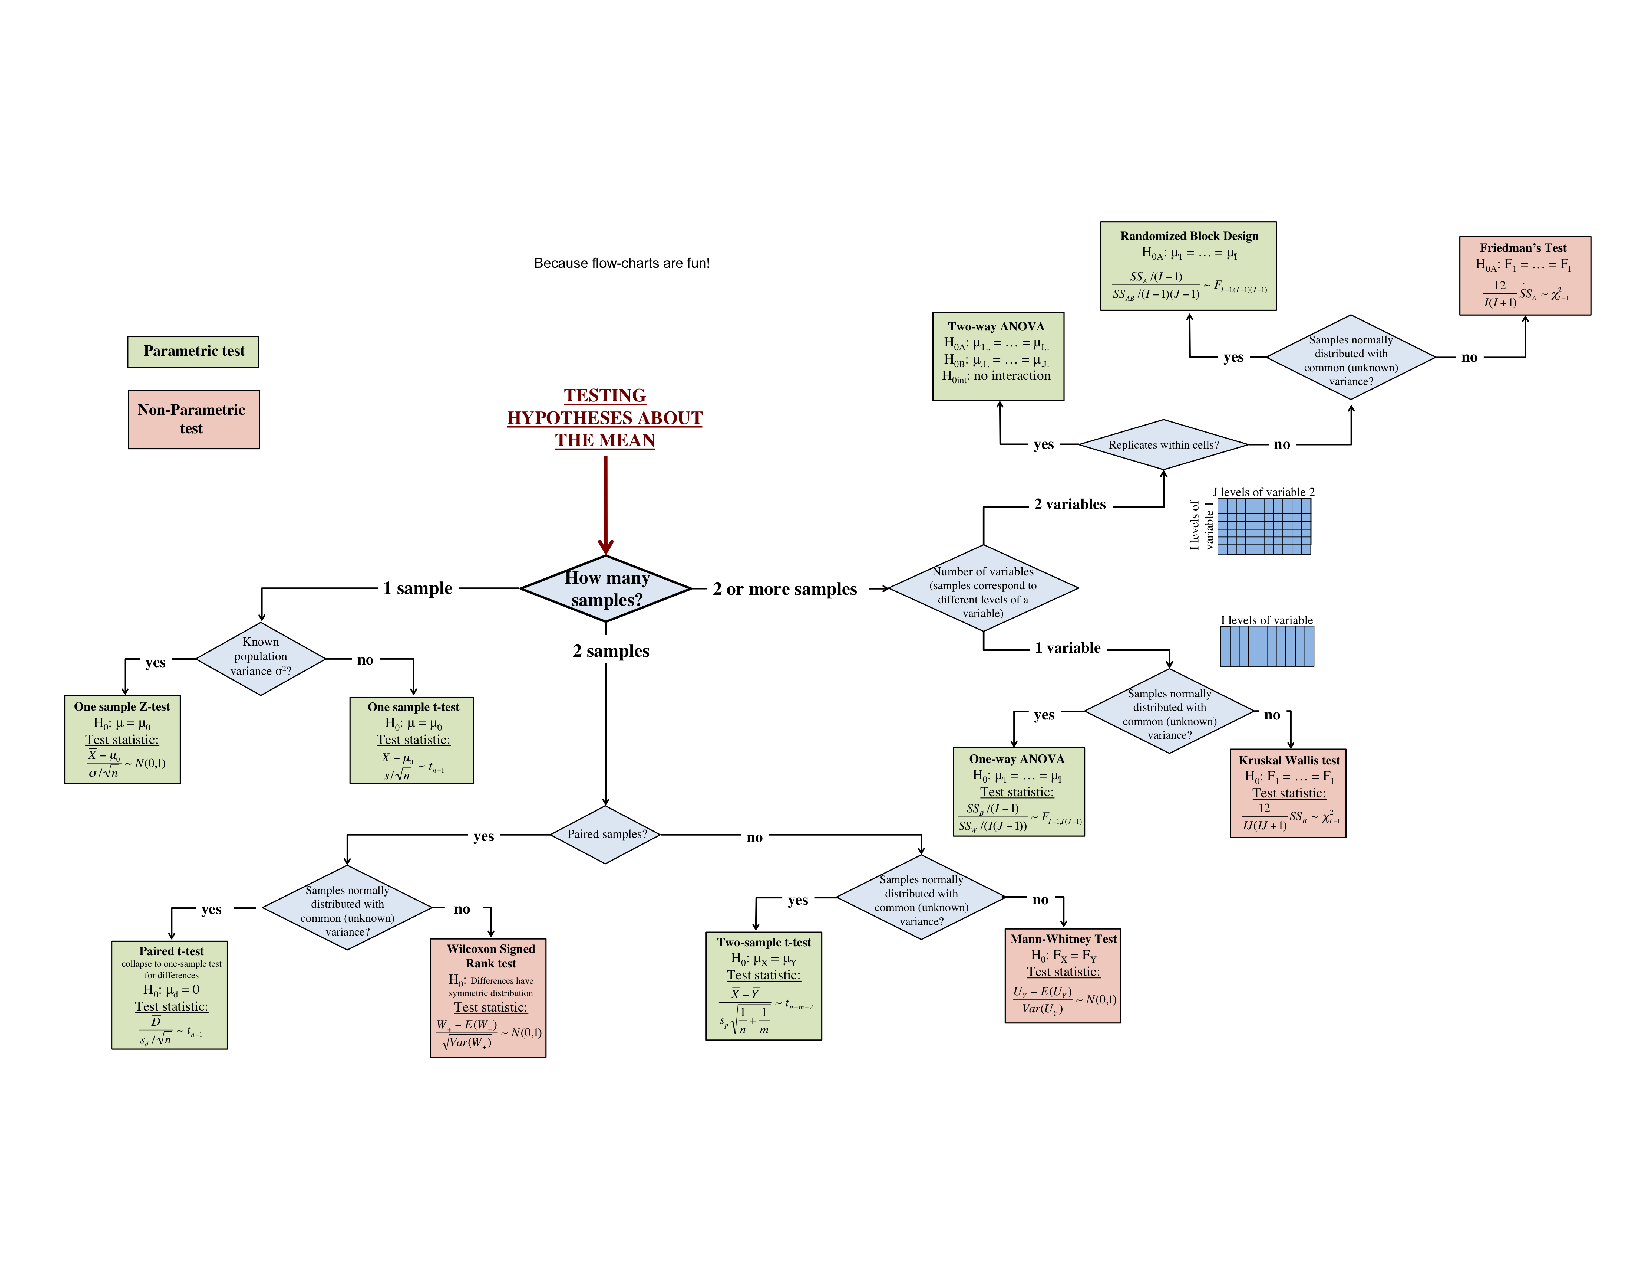
\includepdf[pages=-]{hypothesis_testing_flow_mean.pdf}



\end{document}
